%%%%%%%%% MASTER -- compiles the 4 sections

\documentclass[11pt,letterpaper]{article}

%%%%%%%%%%%%%%%%%%%%%%%%%%%%%%%%%%%%%%%%%%%%%%%%%%%%%%%%%%%%%%%%%%%%%%%%%
\pagestyle{plain}                                                      %%
%%%%%%%%%% EXACT 1in MARGINS %%%%%%%                                   %%
\setlength{\textwidth}{6.5in}     %%                                   %%
\setlength{\oddsidemargin}{0in}   %% (It is recommended that you       %%
\setlength{\evensidemargin}{0in}  %%  not change these parameters,     %%
\setlength{\textheight}{8.5in}    %%  at the risk of having your       %%
\setlength{\topmargin}{0in}       %%  proposal dismissed on the basis  %%
\setlength{\headheight}{0in}      %%  of incorrect formatting!!!)      %%
\setlength{\headsep}{0in}         %%                                   %%
\setlength{\footskip}{.5in}       %%                                   %%
%%%%%%%%%%%%%%%%%%%%%%%%%%%%%%%%%%%%                                   %%
\newcommand{\required}[1]{\section*{\hfil #1\hfil}}                    %%
\renewcommand{\refname}{\hfil References Cited\hfil}                   %%
\bibliographystyle{abbrvnat}                                              %%
%%%%%%%%%%%%%%%%%%%%%%%%%%%%%%%%%%%%%%%%%%%%%%%%%%%%%%%%%%%%%%%%%%%%%%%%%

%PUT YOUR MACROS HERE
\usepackage{change page} % for indentation of sections
\usepackage{lipsum}
\usepackage{hyperref} %for urls
\usepackage{graphicx} %for includegraphics
\usepackage[table]{xcolor} %for table line color alteration
\usepackage{enumitem}  %fancy enumerated lists
\usepackage{wrapfig} %wrap text around figures
\usepackage[leftcaption]{sidecap} % side captions
\sidecaptionvpos{figure}{c} %position side caption
\usepackage[colorinlistoftodos]{todonotes} % comments in margins
\usepackage[round,authoryear]{natbib} %biblio format!
%\usepackage[]{natbib}
%\bibpunct[; ]{[}{]}{,}{n}{}{;} 
%\bibliographystyle{unsrtnat}
\usepackage{multirow} %multirow tables
\usepackage{booktabs} %funky tabs in tables
\definecolor{flame}{rgb}{0.89, 0.35, 0.13}
\definecolor{glaucous}{rgb}{0.38, 0.51, 0.71}
\newcommand{\jri}[1]{\todo[size=\scriptsize, color=flame]{#1}}
\newcommand{\mbh}[1]{\todo[size=\scriptsize, color=glaucous]{#1}}
\renewcommand{\thesubsection}{Objective \Roman{subsection}}
\renewcommand{\thesubsubsection}{\thesubsection\Alph{subsubsection}}
\renewcommand{\theenumi}{\Alph{enumi}}
\newcommand{\zp}{\emph{parviglumis}}
\newcommand{\zpp}{\emph{perennis}}
\newcommand{\zd}{\emph{diploperennis}}
\newcommand{\zl}{\emph{luxurians}}
\newcommand{\zm}{\emph{mexicana}}
\newcommand{\zh}{\emph{huehuetenangensis}}

%\includeonly{NSFsumm}

\begin{document}
%%%%%%%%%%%%% Project Summary max 1 page must include Intellectual Merit and Broader Impact) %%%%%%%%%%%%%%%%%%%
\setcounter{page}{1}
%%%%%%%%% PROJECT SUMMARY -- 1 page, third person
% e.g:  "The PI will prove" not "I will prove"

%Below are the pagination, font size, spacing and margin
%instructions for NSF proposals: \\
%
%FastLane does not automatically paginate a proposal.
%Each section of the proposal must be individually
%paginated prior to upload to the system. \\
%
%Use Computer Modern family of fonts at a font size of 11 points or
%larger. A font size of less than 10 points may be used for mathematical
%formulas or equations, figure, table or diagram captions and when
%using a Symbol font to insert Greek letters or special characters.
%The text must still be readable. The use of small type not in compliance with the NSF guidelines
%may be grounds for NSF to return the proposal without review. \\
%
%No more than 6 lines of text within a vertical space of 1 inch. \\
%
%Margins, in all directions, must be at least an inch. \\
%
%
\required{Project Summary}

\paragraph{Overview} The proposed project will investigate the genome-wide effects of hybridization and introgression in the genus \emph{Zea}.  First, investigators will study two independent hybrid zones that naturally occur in mid-elevations of Mexico between the lowland-adapted \emph{Z. mays} ssp. \emph{parviglumis} (hereafter, \emph{parviglumis}) and the highland-adapted \emph{Z. mays} ssp. \emph{mexicana} (hereafter, \emph{mexicana}).  Through field collections, generation of phenotypic data in common garden studies, and genotyping, the investigators will assess how fitness of these taxa varies across a hybrid zone, the level of convergence in the genetic architecture of introgression across independent hybrid populations and zones, and the evidence for selection on putatively adaptive phenotypic traits across an elevation gradient. Second, investigators will determine the impact of hybridization and introgression between domesticated maize (\emph{Z. mays} ssp. \emph{mays}) and wild  \emph{Zea} as maize spread from its center of origin. Population genomic analyses of sympatric collections will be used to test hypotheses about the significance of divergence time in patterning introgression between these taxa, the geographic scale of adaptive introgression, and the potential for maize, a widespread taxon, to serve as a bridge for gene flow between otherwise allopatric and narrowly-distributed \emph{Zea} species.

% This should be a brief statement of the problem you plan to address.
% It should look something like an abstract. 

%The project summary should be a description of the proposed activity suitable
%for publication, no more than one page in length. It should not be
%an abstract of the proposal, but rather a self-contained description of
%the activity that would result if the proposal were funded. The summary
%should be written in the third person and include a statement of objectives
%and methods to be employed. It should be informative to other persons
%working in the same or related fields and understandable to a scientifically
%or technically literate lay reader. \\
%
%The summary must clearly address in separate statements (within the one-page summary):
%the intellectual merit of the proposed activity; and the broader impacts
%resulting from the proposed activity. Proposals that do not separately
%address both criteria within the one-page Project Summary will be returned without
%review. \\

\paragraph{Intellectual Merit}  Much progress has been made in the study of hybridization and introgression through the development of theory, through field-based ecological research, and through genetic analyses based on a limited number of molecular markers. However, much remains to be discovered regarding how these evolutionary processes have shaped genomes. The research proposed here will leverage the genomic resources of the maize model system to investigate how hybridization and introgression have molded the genomes of both wild \emph{Zea} species and domesticated maize by 1) Generating novel diversity that has potentially been adaptive in two independent hybrid zones of \emph{parviglumis} and \emph{mexicana}; and 2) Facilitating the spread of maize across the Americas through transference of local adaptation from local wild species to maize. These investigations will generate basic knowledge on the level of convergence in introgression in replicate hybrid zones and the role of introgression in facilitating rapid local adaptation during the spread of a colonizing species.

% This is why your project is interesting and will help further
% knowledge in the field of mathematics. 

%How important is the proposed activity to advancing
%knowledge and understanding within its own field or across different fields?
%How well qualified is the proposer (individual or team) to conduct the project?
%(If appropriate, the reviewer will comment on the quality of prior work.)
%To what extent does the proposed activity suggest and explore creative, original,
%or potentially transformative concepts? How well conceived and organized is the
%proposed activity? Is there sufficient access to resources?  \\

\paragraph{Broader Impacts}

The investigators will achieve societally relevant outcomes in the proposed project by providing STEM training opportunities for undergraduate and graduate students and establishing an exchange program between universities in the United States and Mexico.
The investigators have an excellent track record of providing training opportunities for both undergraduate and graduate students in laboratory, computational, and field-based research, have successfully recruited minority students into their research programs in the past and will make every effort to do so as part of this proposed work.
In addition, a teaching module on hybridization will be developed for the undergraduate core course "Principles of Biology" at Iowa State University based on the research proposed here.
This module will actively engage undergraduates in STEM-based research and will serve as a recruiting tool for independent research supported by this project in the investigators' laboratories.
Finally, a proposed exchange program will create an opportunity for students from the United States to conduct research internationally and allow these students to interact with visiting students from Mexico. Through these interactions, students will be better prepared for modern STEM research, which is often highly collaborative and international in nature.

% There are 4 kinds of broader impacts.
% 1. advance discovery and understanding while promoting teaching,
% training and learning
% 2. broaden the participation of underrepresented groups
% 3. disseminated broadly to enhance scientific and technological
% understanding
% 4. benefits of the proposed activity to society% Max 1 page
%%%%%%%%%%%%%
 %Project Description max 15 pages (usually) Must include discussion of recent Prior (last 5 years) %%%%%%%%%%%%%%%%%%%
\setcounter{page}{1}
%%%%%%%%% PROJECT DESCRIPTION  -- 15 pages (including Prior NSF Support)

\required{Project Description}
\begin{center}
%\emph{Maximum of 15 pages}
\end{center}
%The Project Description (including Results from Prior NSF Support, which is
%limited to five pages) may not exceed 15 pages. Visual materials, including charts,
%graphs, maps, photographs and other pictorial presentations are included in the
%15-page limitation. PIs be cautioned that the project description must
%be self-contained and that URLs that provide information related to the proposal
%should not be used. \\
%
%All proposals to NSF are reviewed utilizing the two merit review criteria,
%intellectual merit and broader impacts. \\
%
% The Project Description should provide a clear statement of the work 
% to be undertaken and must include: objectives for the period of the proposed 
% work and expected significance; relation to longer-term goals of the PI's 
% project; and relation to the present state of knowledge in the field, 
% to work in progress by the PI under other support and to work in progress 
% elsewhere.

%%%%%%%%%%%%%%%%%%%%%%%%%%%%%%%%%%%%%%%%%%%%%%%%%%%%%%%%%%%%%%%%%%%%%%
%INTRO
%%%%%%%%%%%%%%%%%%%%%%%%%%%%%%%%%%%%%%%%%%%%%%%%%%%%%%%%%%%%%%%%%%%%%%
\section*{Introduction}

While the potential role of hybridization and introgression as agents of evolution has long been postulated \citep{Anderson1948, Anderson1954, Stebbins1959}, only recently have technological innovations allowed for characterization of these processes on a genome-wide scale. 
Multiple studies have now reported evidence of inter-taxon introgression in both plant \citep{Hufford2013, renaut2013} and animal \citep{consortiumbutterfly2012, staubach2012, huerta2014} species based on full-genome data.
Genomic tools provide the capacity to evaluate the genomic extent of introgression, differentiate neutral from adaptive introgression, and evaluate whether distinct hybrid populations show convergent patterns of introgression.
With this expanded perspective, we can fully evaluate hypotheses first articulated by \citet{Anderson1954}: that 1) Evolution can occur rapidly through selection on novel variation generated by hybridization, and 2) The shuffling and redistribution of previously isolated species through anthropogenic activity has provided ample opportunity for hybridization to occur \citep{Anderson1954}.
Given its evolutionary history and vast genomic resources (\emph{e.g.}, functional annotations, reference genomes, haplotype maps, knock-out libraries), the \emph{Zea} study system represents an unparalleled opportunity for testing these hypotheses and realizing the promise of genomic data for hybridization studies. 

In the investigation proposed here, we will build upon our previous work in maize (\emph{Zea mays} ssp. \emph{mays}) and its wild relatives the teosintes (\emph{Zea} spp.) to characterize the evolutionary role of hybridization and introgression in this system. 
Within \emph{Zea} we will conduct a genomic assessment of these processes in two distinct settings:  
First, analysis of hybridization in two parapatric and uniquely-adapted teosinte subspecies will allow us to answer quetions about convergent introgression and the extent to which selection determines patterns of gene flow.
Second, evaluation of introgression between maize and teosinte outside the domestication center will inform our understanding of the importance of adaptive introgression during colonization of novel environments and test the role of widespread species to act as bridges for gene flow among their congeners.

This proposal builds considerably upon a previous full submission to the 2014 NSF-DEB competition that was favorably reviewed but not funded due to concerns over certain aspects of experimental design that we have rectified here.
In addition, over the last year we have conducted further preliminary analysis, solidified collaborations with colleagues in Mexico and Guatemala, and ensured that this project is logistically feasible.

%%%%%%%%%%%%%%%%%%%%%%%%%%%%%%%%%%%%%%%%%%%%%%%%%%%%%%%%%%%%%%%%%%%%%%
%OBJECTIVES
%%%%%%%%%%%%%%%%%%%%%%%%%%%%%%%%%%%%%%%%%%%%%%%%%%%%%%%%%%%%%%%%%%%%%%
\section*{Objectives}
	
%We will leverage the resources of the \emph{Zea} study system to address two primary objectives:

\subsection*{Objective I: Assess the evolutionary role of hybridization in locally-adapted, parapatric wild teosinte}
\emph{Zea mays} ssp. \emph{parviglumis} (the wild progenitor of maize; hereafter, \emph{parviglumis}) and \emph{Zea mays} ssp. \emph{mexicana} (hereafter, \emph{mexicana}) diverged approximately 60,000 BP \citep{Ross-Ibarra2009a} and have parapatric distributions: while \emph{parviglumis} occurs in the warm lowlands of southwest Mexico, \emph{mexicana} is found in the cool highlands of the Central Plateau. 
Narrow regions of admixture between these wild subspecies have been discovered at middle elevations \citep{Fukunaga2005, Pyhajarvi2013}. 
Through targeted collections, high-density genotyping, population genomic analyses, and common garden experiments, we will address the following research questions: 
%\jri{in general i like the idea of rephrasing questions in terms of concrete hypotheses: ideas we can support or reject. the problem with things like ``what fraction of the genome'' is that you'll always get a number, but it's not clear what that number really means. so what if it's 47\%? instead, if we phrase as a hypothesis that can be tested with a percentage, i think that's much nicer.  So maybe genome congealing proposes that the only gene flow we should see is in high recombination regions.  we can test that, with the same exact methods etc.}

\begin{enumerate}
\item \emph{Do independent hybrid zones show convergent or unique patterns of introgression?}
%\jri{can we phrase this as i did in the intro as convergence of patterns of introgression? make the argument as people do for convergent evolution studies that seeing the same loci introgress always sorta kinda has to imply selection.} 

\item \emph{Do hybrid populations show higher fitness than parental subspecies in some environments?}
%\jri{was trying to think of how to make this more in line with tension/ecotone. i think switching intermediate with some does it. if hybrid pops never show higher fitness, tension zone. if they show fitness in at least some environs, you can argue ecotone. thoughts?}

\item \emph{Is there evidence of selection on putatively adaptive phenotypes across hybrid zones?} 
\end{enumerate}

\subsection*{Objective II: Determine the extent to which anthropogenic movement of maize has enabled hybridization among taxa in \emph{Zea}}
%Determine the extent to which hybridization and introgression have altered the \emph{Zea} genus during the post domestication spread of maize}
Maize was domesticated in southwest Mexico from \emph{parviglumis} $\sim$9,000 BP \citep{Matsuoka2002} and quickly spread throughout the Americas, bringing this crop into sympatry with new species of teosinte \citep{Vigouroux2008a}. 
Through a combination of dense genotyping of range-wide samples of maize and teosinte and targeted, full-genome sequencing we will assess three questions regarding the importance of introgression during the spread of maize:
\begin{enumerate}
\item \emph{Does hybridization with locally-adapted relatives facilitate the spread of an invading species?} \jri{not sure i like this but i want to rephrase these questions in more general terms like the ones you have above, rather than maize-specific}
%\item \emph{Was the spread of maize facilitated by gene flow from locally-adapted wild \emph{Zea}?} \jri{maybe redo as does gene flow from local facilitate spread of invader?}
\mbh{I think it works..."invading" is kind of a loaded term though...a species has to fulfill a list of criteria to be characterized as invasive including negative societal impacts and effects on native species.  Might be better to rephrase to "spread of a colonizing species".}
\item \emph{Is introgression adaptive on a local scale?}
\item \emph{Can a widespread species serve as a bridge for gene flow among otherwise allopatric taxa?} \jri{again not sure I like but want to make more general. thoughts?} \mbh{yes, keep it general. Reviewers seemed to want to see how this study would be broadly applicable.}
\end{enumerate}

%%%%%%%%%%%%%%%%%%%%%%%%%%%%%%%%%%%%%%%%%%%%%%%%%%%%%%%%%%%%%%%%%%%%%%
%RATIONALE AND SIGNIFICANCE
%%%%%%%%%%%%%%%%%%%%%%%%%%%%%%%%%%%%%%%%%%%%%%%%%%%%%%%%%%%%%%%%%%%%%%
\section*{Rationale and Significance}
Pioneers in evolutionary biology including G. Ledyard Stebbins and Edgar Anderson recognized the important role hybridization and introgression could play in adaptation and speciation \citep{Anderson1948, Anderson1954}.
These evolutionary forces were thought to be particularly influential when environmental conditions encountered by a species were marginal, variable, or new \citep{Stebbins1959}.
More recently, defined and stable regions of hybridization, referred to as hybrid zones, have been discovered in a number of taxa \citep[reviewed in ][]{HarrisonHybridZone, shurtliff2013, abbott2014}. 
Increasingly, it is clear that the phenomena of hybridization and subsequent introgression shape genomes and influence the trajectory of species as they evolve \citep{Ellstrand2014}.
Hybridization has long been believed to play a role in speciation, and introgression of even a small number of loci can enable a species to adapt and invade novel habitats \citep{currat2008, abbott2013}.
For example, we now have strong molecular evidence that hybridization has led to speciation in both plants and animals \citep[reviewed in][]{mallet2007} and that colonization events of non-native species \citep{lucek2010} and domesticated crops \citep{he2011, Hufford2013} have been facilitated by introgression. 

While theory regarding hybridization has progressed and many compelling empirical examples have been identified, several outstanding questions remain. 
For example, do neutral tension zone or adaptive ecotone dynamics prevail in hybrid zones \citep{Kruuk1999, Rasmussen2012, Smith2013b}?
If introgression is adaptive, what is the geographic scale of this adaptation?
Are the same adaptive alleles introgressed in independent hybrid populations or are patterns of introgression driven more by local environmental conditions?
Has gene flow from native relatives allowed colonizing species to more readily adapt to new environments?
Can a widespread congener act as a bridge for gene flow between more narrowly distributed allopatric taxa?
Genome-wide analysis of variation in the extent and genetic architecture of introgression --- the number and size of introgressed loci ---  will offer considerable insight regarding these questions.  
For example, the few genomic studies of introgression completed thus far have already suggested that rates of gene flow vary substantially across loci, likely as a function of selection on introgressed alleles \citep{Hufford2013, Poelstra2014}, and that introgression has occurred at genomic locations underlying adaptive phenotypes that may have facilitated colonization of a non-native taxon \citep{Hufford2013}.
 
The \emph{Zea} study system is uniquely suited for pushing the field of hybridization biology forward during the modern genomic era.
The \emph {Zea mays} subspecies \emph{parviglumis} and \emph{mexicana} are distributed across a steep altitudinal gradient and differ for phenotypes that are thought to be adaptive in the highlands such as the presence of macrohairs, stem pigmentation and shorter flowering time in \emph{mexicana}.
A recent ecological niche study has found that the potential distributions of these subspecies are largely allopatric and stable over many thousands of years \citep{hufford2012inferences}.
However, analysis of microsatellite markers genotyped in a range-wide sample has identified elevated admixture between the subspecies in two geographically-distinct, mid-elevation regions of Mexico where the distributions of parental subspecies overlap, suggesting the presence of multiple hybrid zones \citep{Fukunaga2005}.  
Our recent genome-wide analysis of twelve individuals from a population in one of these hybrid zones revealed abundant small blocks of admixture in all individuals, suggesting long-term gene flow between subspecies \citep{Pyhajarvi2013}.  
Very little is known, however, about patterns of introgression across populations in this region or in independent hybrid zones.
By expanding our preliminary studies beyond a single population, we can assess how introgression varies across regions and hybrid zones and determine if specific haplotypes are consistently introgressed and widely adaptive or, rather, tied to specific habitats. \jri{this is well phrased, but then begins to make me think it overlaps with aim 2 of objective 2. basically asking how local adaptive inrogression is. do we play up that parallelism or play it down?} \mbh{my inclination would be to not play it up}

\label{bookmark}
In addition to hybridization between \emph{parviglumis} and \emph{mexicana}, gene flow between domesticated maize and various wild \emph{Zea} has been detected based on both hybrid morphologies observed in the field \citep{wilkes1967teosinte, Wilkes1977} and genetic data \citep{Fukunaga2005,Ross-Ibarra2009a}. 
Maize domestication from \emph{parviglumis} occurred recently on an evolutionary timescale \citep[$\sim$9,000BP;][]{Matsuoka2002} and was followed by rapid spread of the crop across the Americas over the following millennia \citep{Piperno2001,Grobman2012}. 
During this expansion, maize was brought into sympatry with new wild relatives that were likely allopatric to the progenitor of maize (\emph{i.e., parviglumis}) for long periods prior to domestication \citep{hufford2012inferences}. 
Our recent work has provided evidence of introgression from \emph{mexicana} into maize during its colonization of the highlands of the Mexican Central Plateau.  
We found consistent introgression into several highland maize populations at QTL for phenotypes (\emph{e.g.}, pigment and macrohairs) that distinguish highland \emph{mexicana} from lowland \emph{parviglumis} teosinte, and showed that both \zm{} phenotypes and higher growth rate were found in maize plants with \emph{mexicana} introgression \citep{Hufford2013}.
Our interpretation of these results is that maize received adaptive introgression from \emph{mexicana} that allowed the crop to spread into the highlands of Mexico. \jri{should we move some of these sentenes on hufford 2013 down below with objetive 2?} \mbh{I'll leave that up to you...feel free to move them and patch up a transition here it you'd like}

Subsequent to its diffusion into the Mexican highlands, maize spread into sympatry with additional teosinte taxa in Guatemala including \emph{Zea luxurians} (hereafter, \emph{luxurians}) and \emph{Zea mays} ssp. \emph{huehuetenangensis} (hereafter, \emph{huehuetenangensis}), each adapted to environmental conditions very different from those of the progenitor \emph{parviglumis}. 
Although maize is known to hybridize with both taxa, the extent and adaptive significance of gene flow between these teosintes and maize is unknown.  
Additionally, based on analysis of a small number of resequenced loci, \emph{mexicana} haplotypes appear to be segregating in \emph{luxurians} \citep{Ross-Ibarra2009a}.  
Since \emph{mexicana} and \emph{luxurians} are entirely allopatric in their distributions, this suggests maize may have served as a bridge for gene flow between these two taxa.  
Further work will be necessary to explore this possibility and to assess if the genomes of \emph{Zea} species have been largely altered through gene flow during the spread of maize across the Americas (see \ref{ss:genuswide}).

%%%%%%%%%%%%%%%%%%%%%%%%%%%%%%%%%%%%%%%%%%%%%%%%%%%%%%%%%%%%%%%%%%%%%%
%SPECIFIC OBJECTIVES
%%%%%%%%%%%%%%%%%%%%%%%%%%%%%%%%%%%%%%%%%%%%%%%%%%%%%%%%%%%%%%%%%%%%%%
\section*{Research Plan}

\subsection{Evolutionary genomics of teosinte hybrid zones}
\label{ss:hybrids}
\subsubsection{What fraction of the genome is porous to gene flow in hybrid zones?}
\label{sss:genomescan}

\jri{reword what fraction question to frame as hypothesis.  i've pasted below in comments text from old preliminary results that i think goes here. i'd keep the figure and drop the table. part b and c of the figure make the point nicely, you can say in text if you want that those are reflected in lower Fst}

%Our previous publications suggest \emph{Zea} is a promising model system for exploring the evolutionary role of hybridization and introgression (\emph{e.g.},  \citealt{Ross-Ibarra2009a, vanheerwaarden2011a, Hufford2013, Pyhajarvi2013}).  To further refine our research questions and provide preliminary results for this proposal we have reanalyzed published data  \citep{Fang2012} of 983 SNPs genotyped across a panel of $>2,000$ samples including all subspecies and species of teosinte and an Americas-wide sample of maize landraces (\emph{i.e.}, traditional open-pollinated varieties).  While the low density of markers in these data precludes genome-wide inferences and haplotype-based analyses, the comprehensive taxon sampling makes this an ideal resource for guiding future research.
%
%\subsection*{Evidence for hybrid zones between \emph{parviglumis} and \emph{mexicana}}
%
%Using the \citet{Fang2012} data, we calculated the probability of each sample's assignment to \emph{parviglumis} and \emph{mexicana} groups using STRUCTURE \citep{Pritchard2000}.  We find that individuals from several mid-elevation populations show appreciable assignment to both \emph{parviglumis} and \emph{mexicana} groups (Figure \ref{fig:structure}) and likely represent hybrid populations.  
%
%\begin{figure}[h!] 
%  \centering
%   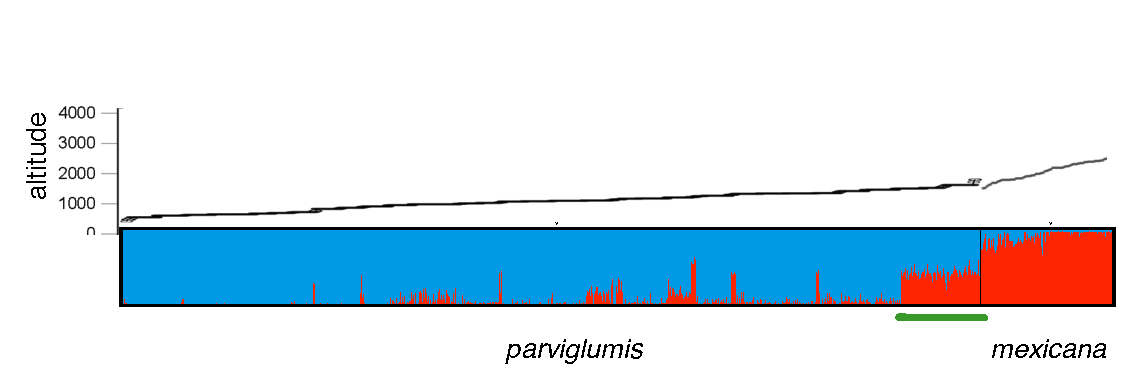
\includegraphics[width=0.95\textwidth]{structure.pdf}
%    \caption{Assignment of \emph{parviglumis} and \emph{mexicana} individuals to K=2 groups using the Bayesian assignment algorithm of STRUCTURE \citep{Pritchard2000}.  Individuals are sorted by increasing altitude as indicated by the plot above the bar chart. Individuals from mid-elevation, hybrid zone populations are underscored in green.} 
%\label{fig:structure}
%\end{figure}
%
%Admixed populations cluster in two geographically distinct regions of Mexico: the eastern Balsas River Basin and eastern Jalisco state.  These locations fall at intermediate locations between the main distributions of \emph{parviglumis} and \emph{mexicana} (Panel A, Figure \ref{fig:pies}).  Hybrid populations from eastern Jalisco state are found at higher elevation (mean 1632m) than those in the eastern Balsas (mean 1531m) and also show a higher proportion of membership in the highland teosinte \emph{mexicana} (Panels B and C, Figure \ref{fig:pies}).  These findings suggest that hybrid populations from distinct environments may vary in the proportion of ancestry from each subspecies in a manner that is adaptive. Estimates of pairwise population differentiation also suggest that hybrid populations in the Balsas and Jalisco are distinct in that Jalisco populations are less differentiated from \emph{mexicana} than hybrid populations in the Balsas (Table \ref{tab:Fst}).  Not surprisingly, populations in both hybrid zones are less differentiated from \emph{mexicana} and \emph{parviglumis} than these subspecies are from each other. 
%
\begin{figure}[h!]
  \centering
   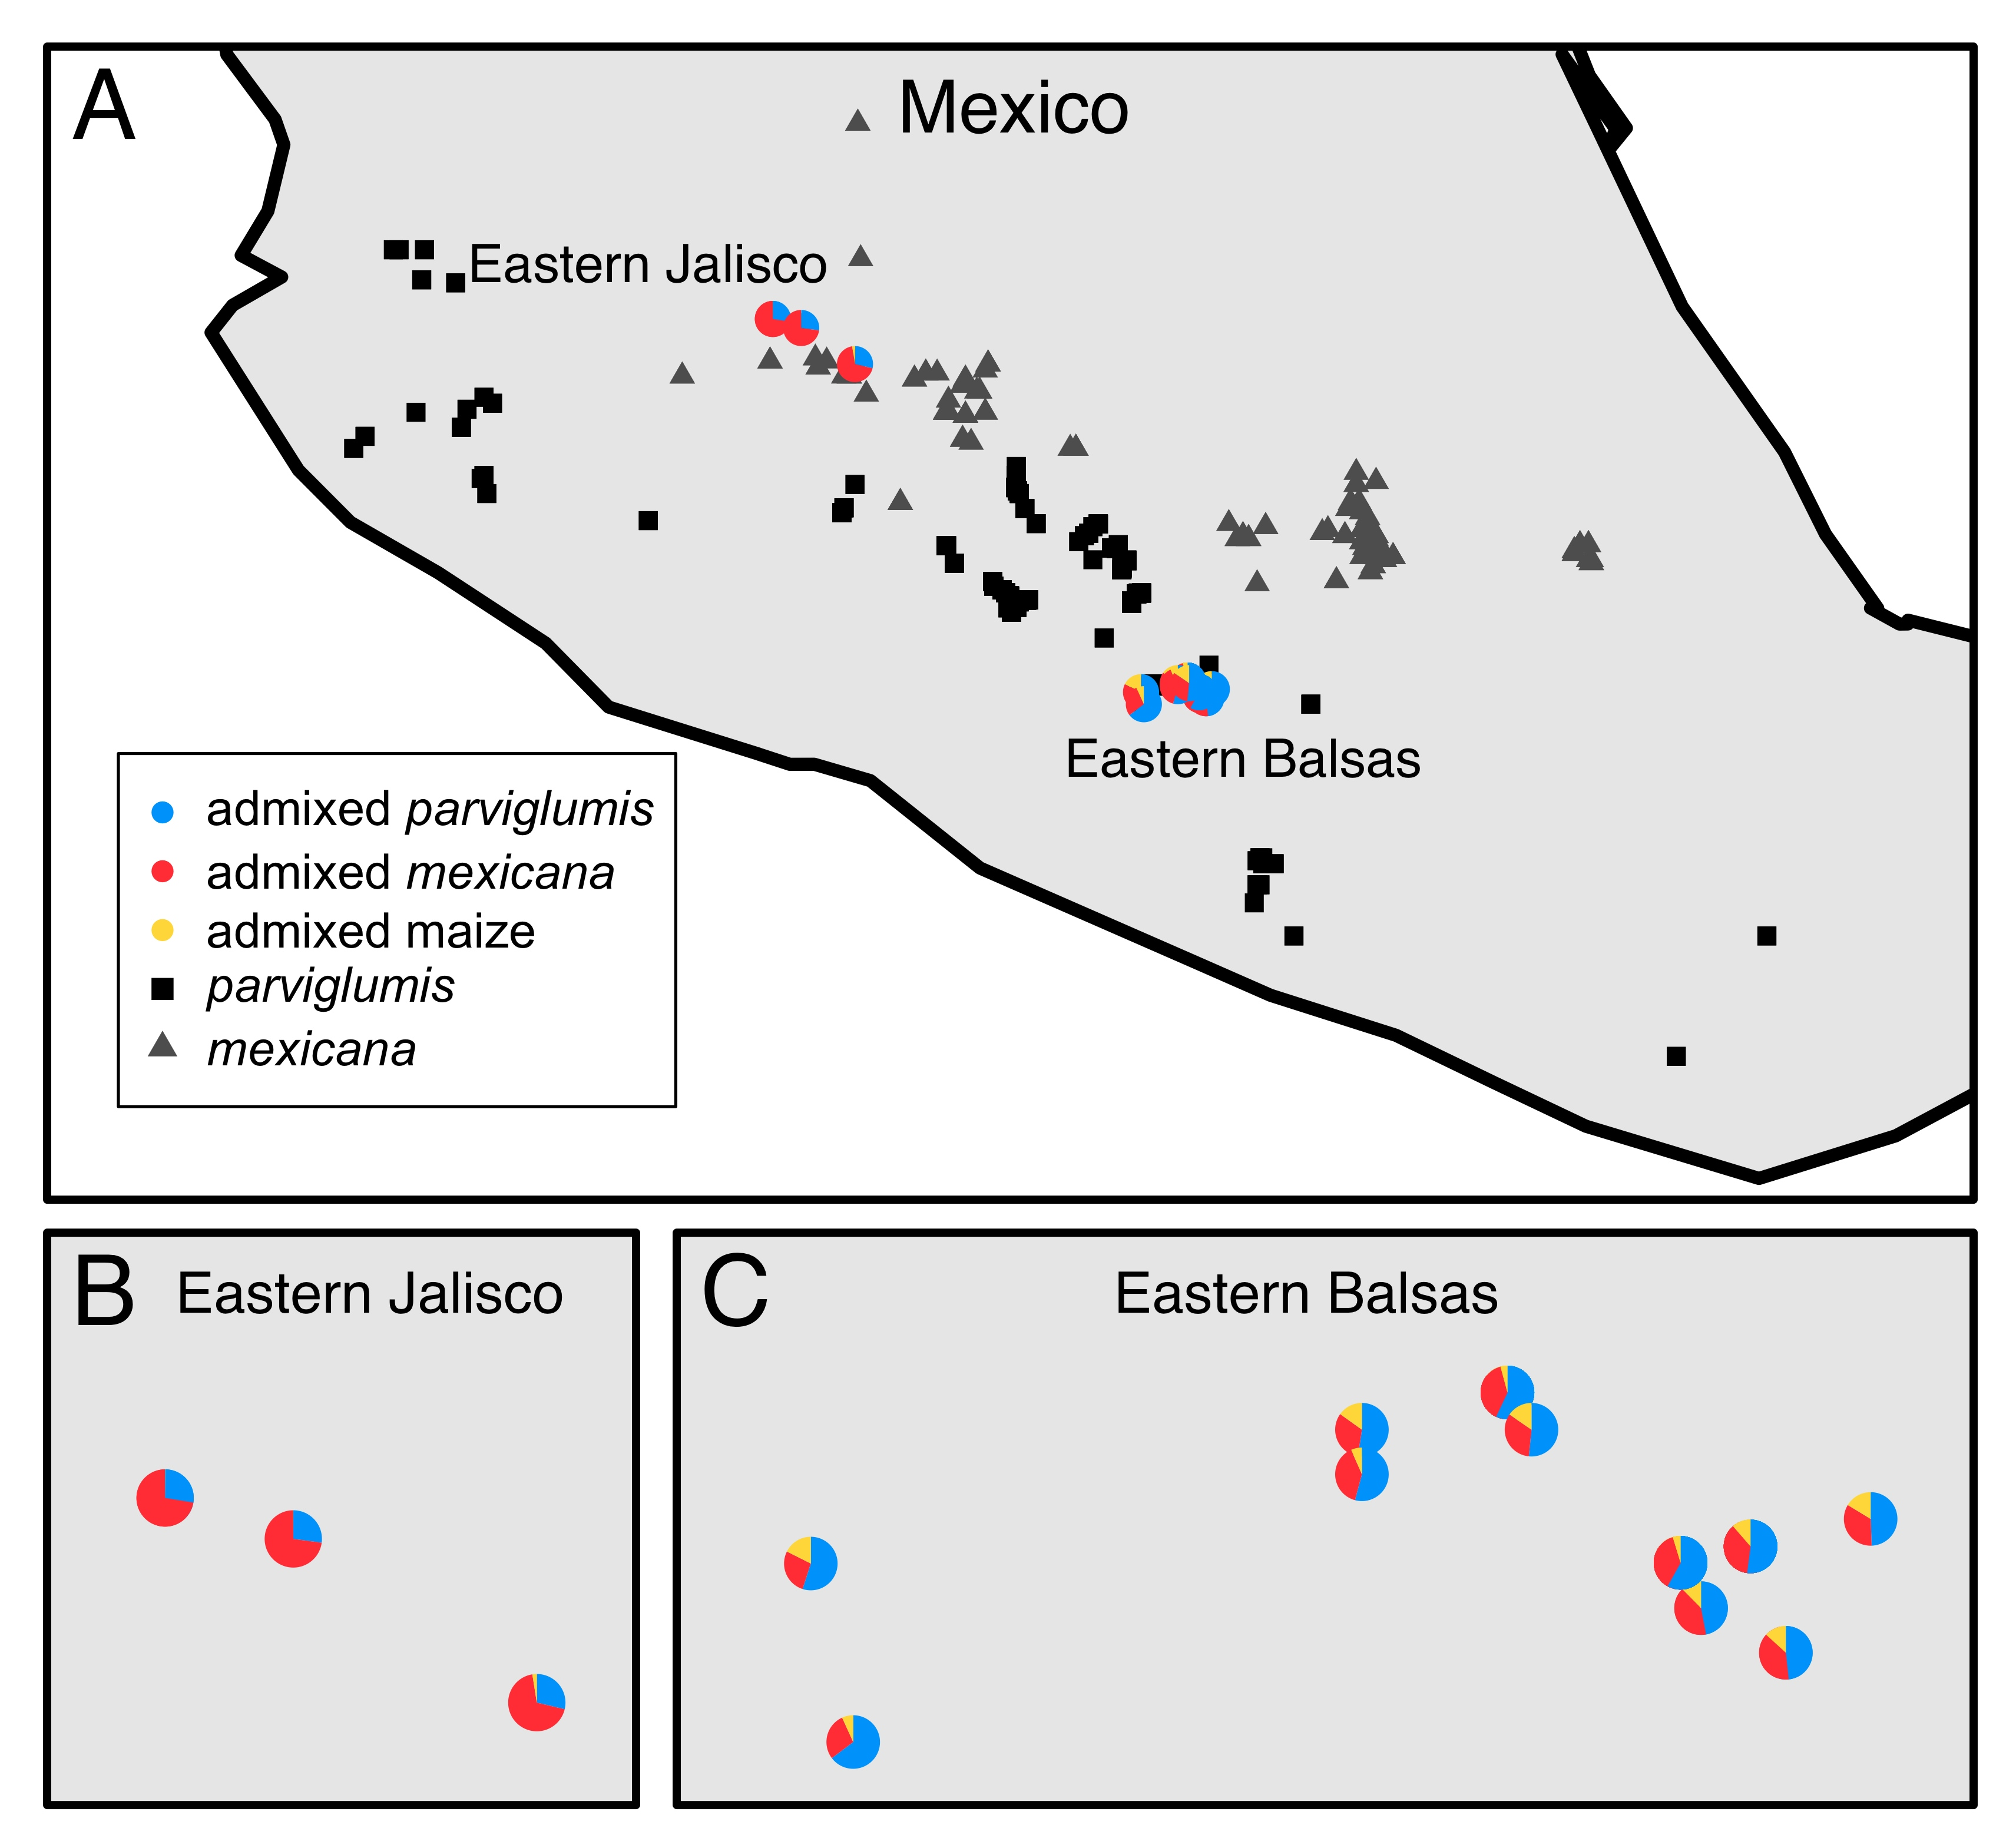
\includegraphics[width=0.7\textwidth]{Figure1.jpg}
    \caption{A) Location of two putative hybrid zones of \emph{mexicana} and \emph{parviglumis}.  Hybrid populations are represented as pie charts with proportion assigned to \emph{mexicana}, \emph{parviglumis}, and maize groups. Zoomed-in views of the Eastern Jalisco (B) and Eastern Balsas (C) hybrid populations.} 
\label{fig:pies}
\end{figure}
%
%\begin{table}[h!]
%\rowcolors{2}{gray!25}{white}
%\begin{center}
%\caption{Pairwise $F_{ST}$ between teosinte and hybrid populations} \label{tab:Fst}
%\begin{tabular}{lcccc}\\\toprule
%{\bf Taxon}&{\bf \emph{parviglumis}}&{\bf \emph{mexicana}}&{\bf Jalisco Hybrids}&{\bf Balsas Hybrids}\\\midrule
%{\bf \emph{parviglumis}}&---&---&---&---\\
%{\bf \emph{mexicana}}&0.107&---&---&---\\
%{\bf Jalisco Hybrids}&0.059&0.064&---&---\\
%{\bf Balsas Hybrids}&0.057&0.074&0.034&---\\\bottomrule
%\end{tabular}
%\end{center}
%\end{table} 
%

Recent studies have suggested the functional architecture of genomes can lead to chromosomal regions of high differentiation in hybridizing species \citep{renaut2013}, but these regions are not always conserved across populations \citep{Parchman2013}. Currently, few studies have dissected the genome-wide architecture of hybridization in replicate hybrid zones, and little is known about the consistency of genome porosity to gene flow. Genome-wide studies in teosinte are feasible at high marker density \citep{Hufford2012b, Hufford2013, Pyhajarvi2013} and are informed by the genomic resources of maize \citep{Hufford2012}, often providing functional annotation for loci of interest, a rarity in other natural systems.  The Hufford Laboratory and Senior Personnel Luis Eguiarte will assess the genomic architecture of hybridization and evidence for selection in two hybrid zones of \emph{mexicana} and \emph{parviglumis} through population collections, generation of genotype and sequence data, and application of population genomic analyses appropriate to this question. 

\paragraph{\emph{Panel Construction and Sample Collection:}}
From previous collections, we have access to an extensive sampling of \emph{parviglumis}, \emph{mexicana}, and maize from throughout their respective ranges.  Moreover, Senior Personnel Luis Eguiarte and collaborator Salvador Montes-Hernandez (see attached letters of commitment) have recently collected altitudinal transects of \emph{parviglumis} and \emph{mexicana} that extend through both hybrid zones targeted by our project \citep{Diez2013} and are  familiar with populations in this region.  Our current collections will likely be insufficient for both the genotyping and common garden activities we propose  and we have therefore budgeted for a collection trip during the first year of the project.  We will collect from 15 sampling sites in each of 16 populations.  Sampling sites will be randomly stratified across the elevation gradient of each population.  At each sampling site we will collect as much seed as possible from each of five teosinte plants.  In the wild, teosinte plants produce an average of $\sim 100$ seeds per plant \citep{wilkes1967teosinte}. 
We will also measure plant density, slope of the terrain, and canopy cover at each sampling site.  These data will be useful covariates for estimating any potential maternal effects in our common garden experiments.  Four populations will be sampled from both the eastern Jalisco and eastern Balsas hybrid zones.  To the extent possible, we will select hybrid populations in a stratified manner across the elevation gradient found in these regions. Four populations each will also be collected from non-admixed \emph{parviglumis} and \emph{mexicana}, with two populations of each taxon collected from regions proximate to both hybrid zones.  We have already obtained the requisite collection permits as well as permits for importing samples into the United States for genetic analysis. Following collection, samples will be sent to the lab of Dr. Eguiarte at the Universidad Nacional Aut\'{o}noma de M\'{e}xico (UNAM) for cold storage until common garden experiments are planted (see \ref{sss:fitness}).  During year two of our proposed project, leaf tissue will be collected from a single plant per sampling site ($n=240$) in our mid-elevation common garden (see \ref{sss:fitness}) at the 5-7 leaf stage, stored in silica, and shipped to Iowa State University for DNA isolations and subsequent genotyping and full-genome sequencing.\jri{FYI silica isn't best for GBS. if possible to ship fresh, better. and remind me to tell you the sampling protocol. if you're doing plates, it will save you billions of years down the road to sample directly into plates correctly in the field}

\paragraph{\emph{Sample Genotyping and Sequencing:}}
DNA for genotyping will be isolated using a modified CTAB procedure \citep{Saghai-Maroof1984}. \jri{another FYI: CTAB sucks for WGS. fine for GBS though} For sample genotyping ($n=240$) we will utilize the services of the Genomic Diversity Facility at Cornell University to implement a reduced representation approach to next-generation sequencing called Genotyping By Sequencing (GBS; \citealt{Elshire2011}; see attached letter of commitment from Dr. Sharon Mitchell). To date, this method has been implemented to genotype tens of thousands of maize samples and a bioinformatics pipeline (TASSLE-GBS) has been constructed that allows for genotyping $\sim$1,000,000 SNPs in maize \citep{Glaubitz2014} using standard GBS data. 
We will multiplex only 48 individuals per lane (instead of the standard 384 used for inbred lines) to minimize missing data and errors in identifying heterozygous genotypes. 
Based on our experience with thousands of diverse maize and teosinte, even after filtering for missing data, GBS provides many more markers with minimal ascertainment bias at a fraction of the cost of other available technologies. 

In addition to GBS data, we will generate full-genome sequence through the Iowa State University DNA Facility for a single hybrid individual from each hybrid zone.  We will generate two lanes of Illumina HiSeq 150bp, paired-end data per individual.  
We have previous experience dealing with whole genome shotgun data \citep{Gore2009,Chia2012a,Hufford2012b}, and have recently developed and implemented an open-source pipeline for read-mapping and SNP calling (\url{https://github.com/RILAB/paap}) using the existing maize B73 reference genome. \jri{bad news: nobody in my lab can get that damn pipeline working. i haven't tried myself. leave it in for now, just another FYI}

\paragraph{\emph{Population Genomic Analyses:}} 
We will assess the genome-wide patterns of ancestry using several approaches.  
First, standard measures of differentiation including $F_{ST}$, the proportion of shared and fixed variants, and relative levels of nucleotide diversity \citep{Geneva2014} will be calculated in sliding windows along the genome. 
Second, we will attempt to implement haplotype-based methods for detecting introgression \citep[\emph{e.g.},][]{price2009, lawson2012} that will effectively allow us to model chromosomes from hybrid populations as mosaics of reference allopatric populations of \emph{parviglumis} and \emph{mexicana}.  
Finally, if phasing genotypes \citep{scheet2006fast} proves difficult given high levels of missing data or heterozygous error, we will make use of software designed to estimate admixture from genotype-likelihoods calculated on low-coverage sequence data \citep{skotte2013estimating}. 
We have already designed pipelines to work with genotype-likelihoods (e.g. \url{https://github.com/arundurvasula/angsd-wrapper}) and can utilize these methods to calculate standard diversity statistics.  
We will evaluate excess of \emph{parviglumis} or \emph{mexicana} ancestry on a site-by-site basis across hybrid genomes at the population level and will determine whether patterns are conserved across populations within hybrid zones and between hybrid zones.  Chromosomal regions showing an excess of ancestry from one taxon in hybrid populations will be inspected for evidence of selection using a combination of site-frequency-, linkage-disequilibrium-, and population-differentiation-based methods \citep[reviewed in][]{Vitti2013}. Chromosomal regions showing strong evidence of selection across individuals within a hybrid zone based on analysis of GBS data will be inspected in our whole-genome resequencing data to refine haplotype boundaries. 
Whole genome sequence data will also allow estimation of the age of the introgression and potentially identifying candidate causal polymorphisms.  

\subsubsection{How do the fitness of parental and hybrid populations vary across the hybrid zone?} 
\label{sss:fitness}
In order to assess fitness and variation at putatively adaptive phenotypes across both non-admixed and  hybrid populations we will conduct common garden experiments in Mexico at three altitudes: 1) Below a hybrid zone in habitat occupied by non-admixed \emph{parviglumis}; 2) Within hybrid zone habitat; and 3) Above a hybrid zone in habitat occupied by non-admixed \emph{mexicana}. 
Common garden experiments will be replicated over years two and three of our proposed project.  

Discussions with collaborators in Mexico (Ruairidh Sawers and Salvador Montes-Hernandez; see attached letters of commitment) raised concerns about the safety of students at field sites in the state of Guerrero (the location of the eastern Balsas hybrid zone; see US State Department Travel Warning at \url{http://travel.state.gov/content/passports/english/alertswarnings/mexico-travel-warning.html}) and the feasibility of managing six concurrent gardens. We thus propose a single transect of three replicate gardens in the eastern Jalisco hybrid zone. 
In our initial discussions with Drs. Sawers and Montes-Hernandez we have identified potential high- and low-elevation sites near Celaya and Bucerias, Mexico respectively.  
We will explore options for our third hybrid zone garden during our collections in the first year of the project.
The hybrid zone is less than 50 kilometers from the host institution of Dr. Sawers (Langebio in Irapuato, Mexico) and identification of an appropriate site should be straight-forward.
Each garden will consist of three complete blocks including a randomization of three plants from each of 15 sampling sites in the 16 populations described in \ref{sss:genomescan} (3 blocks x 3 plants x 15 sites x 16 populations = 2,160 plants per garden).  We will measure fitness-related phenotypes (percent germination, germination rate, plant height at 15-day intervals, seed set, 50-seed weight, total-above-ground biomass, stomatal conductance and survival), putatively adaptive phenotypes across the altitudinal gradient (macrohair density, pigmentation extent, and flowering time) and phenotypes for which there is no \emph{a priori} evidence of selection across an elevational gradient (culm diameter and the width of the leaf beneath the first lateral branch at the time of flowering).  \jri{culm diameter is associated with Inv1n which shows strong altitudinal clines -- see Zhou's paper. i've never looked to see if the phenotype shows a cline but based on that i suspect it might!}
Analysis of relative fitness of hybrid and parental plants across our garden sites will provide evidence regarding ecotone vs. tension zone dynamics in teosinte hybrid zones.  Ecotone dynamics would be supported by hybrids possessing the highest fitness of all plants in the mid-elevation gardens, whereas tension zone dynamics would be supported by hybrids having lower fitness in all gardens.  Phenotypic data for putatively adaptive traits and traits with no evidence of selection will be analyzed in \ref{sss:driftsel}. \jri{other thoughts: 1) somewhere here you need to say these are half-sib families so you can do qst-fst style analyses. do you want to explain qst-fst approaches? 2) if these are half sib families and you think you'll have a reasonable proportion of selfs, we have code that can impute and phase mom and kids. up to you if worth mentioning; I can provide a github link}
		
{
\color{red}  
\noindent\makebox[\linewidth]{\rule{\linewidth}{0.4pt}}
JRI STOPPED HERE \\
\noindent\makebox[\linewidth]{\rule{\linewidth}{0.4pt}}
}
		
\subsubsection{Is there evidence for selection on putatively adaptive phenotypes across hybrid zones?}
\label{sss:driftsel}
Stem pigmentation, macrohair density, and flowering time in particular are thought to be under selection in teosinte across an elevational gradient.  Pigmented and pilose plants have an advantage in retaining heat at high elevation (for a discussion of highland adaptation in the context of maize see \citealt{Eagles1994}). Additionally, \emph{mexicana} flowers much earlier than \emph{parviglumis} \citep{Rodriguez2006}, which may represent an adaptation to shorter growing seasons at high elevation. We will combine our genome-wide marker data obtained in \ref{sss:genomescan} with phenotypic data collected in our common garden experiments in \ref{sss:fitness} in order to evaluate evidence for selection on these potentially adaptive phenotypes.  A method recently developed by \citet{Ovaskainen2011} and implemented in the software DRIFTSEL \citep{Karhunen2013} is particularly suited to this purpose.  The method builds upon the $F_{ST}$--$Q_{ST}$ framework for comparison of population differentiation and quantitative phenotype divergence and allows the signature of selection on a given phenotypic trait to be distinguished from genetic drift.  The strength of evidence for selection based on DRIFTSEL for putatively adaptive phenotypes (pigment, macrohairs, flowering time) will be compared to that of phenotypes with no \emph{a priori} evidence of selection across an elevational gradient (culm diameter and leaf width).

In addition, we will conduct association analyses to connect genotype to phenotype using GBS data described in \ref{sss:genomescan} and phenotypic data for potentially adaptive traits and traits gauging fitness.  Association analysis will be conducted using TASSEL5.0 \citep{Bradbury2007}. Significant associations will then be cross-referenced with regions of excess ancestry from \emph{parviglumis} or \emph{mexicana} in hybrid populations and zones identified in \ref{sss:genomescan}, particularly those that show evidence of selection based on additional population genetic summary statistics.  This final combination of data and analyses could reveal the phenotypes, loci, and ancestry source under selection within hybrid zones.

\subsection{Crop-wild introgression during maize diffusion} \label{ss:genuswide}

%\jri{i like having an intro that ties together the questions. i think some of the text from rational could go here and in your objective 1 above. i still think the rational/significance should address not what the questions are in teosinte per se, but WHY these questions are of interest to a broader audience. for example, i think the scale of adaptive introgression and local adaptation is broadly of interest, as is how repeatable evolution is across replicate hybrid zones. in the rationale and signficance section we only need motivate the reader that these are cool questions; there they can trust us that these questions apply to teosinte.  then, in the objectives below, we give them the relevant background so they can put those cool questions in context for our study. thoughts?}

%\subsection*{Objective II: Determine the extent to which anthropogenic movement of maize has enabled hybridization among taxa in \emph{Zea}}
%%Determine the extent to which hybridization and introgression have altered the \emph{Zea} genus during the post domestication spread of maize}
%Maize was domesticated in southwest Mexico from \emph{parviglumis} $\sim$9,000 BP \citep{Matsuoka2002} and quickly spread throughout the Americas, bringing this crop into sympatry with new species of teosinte \citep{Vigouroux2008a}. 
%Through a combination of dense genotyping of range-wide samples of maize and teosinte and targeted, full-genome sequencing we will assess three questions regarding the importance of introgression during the spread of maize:
%\begin{enumerate}
%\item \emph{Does hybridization with locally-adapted relatives facilitate the spread of an invading species?} \jri{not sure i like this but i want to rephrase these questions in more general terms like the ones you have above, rather than maize-specific}
%%\item \emph{Was the spread of maize facilitated by gene flow from locally-adapted wild \emph{Zea}?} \jri{maybe redo as does gene flow from local facilitate spread of invader?}
%\item \emph{Is introgression adaptive on a local scale?}
%\item \emph{Can a widespread species serve as a bridge for gene flow among otherwise allopatric taxa?} \jri{again not sure I like but want to make more general. thoughts?}
%\end{enumerate}




Following domestication, maize spread rapidly across the Americas, colonizing novel environments different from that inhabited by its wild ancestor \zp. 
During this diffusion, maize came in contact with each of the other wild teosinte taxa in the genus \emph{Zea}.  
Hybridization between maize and each of these taxa has been previously documented \citep[see][for a review]{doebley1990molecular}, raising a number of questions about the role of gene flow in the recent evolution of both maize and its wild relatives.
In this objective, the Ross-Ibarra Laboratory  will address three questions that arise from this natural experiment.  
First, given previous evidence of the potentially adaptive significance of introgression from the teosinte \zm, we ask whether maize colonization of the tropical lowlands of Guatemala was also facilitated by adaptive introgression from the teosintes \zl{} and \zh.
Second, building on our previous observations in the highlands of the Central Plateau, we seek to define the geographic scale over which introgression may be adaptive.
Finally, we return to the observation of haplotype sharing between allopatric teosinte taxa \citep{Ross-Ibarra2009a} and propose to test whether these results are best explained by incomplete lineage sorting or the possibility that domesticated maize may have served as a bridge for indirect gene flow among teosinte populations. 

\subsubsection{Do the fitness consequences of gene flow from locally adapted populations depend on divergence?}
\label{sss:adaptive_intro}


%Does gene flow facilitate colonization/invasion?"
%if it always does, then we expect to see lux as well as mex
%if the answer is "it depends" -- on genetic distance, habitat, DMI, whatever, then maybe we won't see it

Maize was domesticated from \zp\ in the Balsas River valley on the Pacific Coasts of Mexico.  
As maize spread from its center of origin, it encountered and adapted to a wide range of different environments.

We have previously documented the importance of introgression in facilitating maize adaptation to the highlands of the Mexican Central Plateau \citep{Hufford2013, Takuno15062015}.
As maize spread from its origins in the Pacific Coast of Mexico, it  encountered a number of different environments in addition to the highlands.
By only a few thousand years after domestication, for example, maize had arrived in the humid lowlands of Guatemala \citep{neff2006early}.  
Conditions in Guatemala are substantially more tropical than the southwest coast of Mexico inhabited by \zp, with warmer winters, lower annual fluctuation in temperature, and more than double the annual precipitation.
Upon arrival in Guatemala, maize came into contact with the wild teosintes \zh{} and \zl.  
These taxa exhibit a number of adaptations to their environment including differences in root architecture, flooding tolerance, and delayed flowering \citep{wilkes1967teosinte, mano2006}.
Maize is known to hybridize with both taxa \citep{wilkes1967teosinte}, raising the possibility that the process of adaptive introgression we observed in the highlands of Central Mexico is mirrored in the humid lowlands of Guatemala.

To address this question we will sample six populations of both \zl{} and \zh{}, stratified across their elevational range in Guatemala.  
Two of these populations will be chosen to be as distant as possible from domesticated maize, and used as a control representative of ancestral haplotypes or allele frequencies.  
For the remaining four populations of each taxon, we will sample populations of both the teosinte and a sympatric or nearby maize landrace population.
Additionally, two maize populations from similar environment, but allopatric to teosinte, will also be chosen, for a total of 24 maize and teosinte populations.
We will be assisted in our collection efforts by Mario Fuentes L\'{o}pez of the Fundit Organization in Guatemala (see attached letter of commitment).
We will genotype 12 individuals from each population using GBS. 
Two individuals (either two \zl\ or one \zl\ and one maize) will be fully sequenced.
There is currently no full genome sequence of \zl, and this will allow us to delineate introgressed or selected regions, identify copy number variants, and potentially identify candidate adaptive polymorphisms within the regions of interest.
Analysis of introgression and selection will follow methods described in \ref{sss:genomescan}.
If introgression from either of these teosintes has been adaptive to colonization of Guatemala, we predict we will find evidence of introgression in the majority of maize populations, that these regions will show evidence of recent selection in maize, and that they will overlap with QTL for phenotypes likely to be adaptive in these environments \citep[e.g.][]{omori2007qtl,mano2008linkage}.
We also predict that the same regions should show evidence of selection against introgression from maize into \zl.
Results from these analyses will help establish whether observations of adaptive introgression from \zm{} are an anomaly unique to the highlands of Mexico, or whether adaptive introgression from crop wild relatives may be a common occurrence that has facilitated the spread of domesticated taxa beyond their original habitat.

Finally, this aim will also provide useful baseline information on patterns of genetic diversity in \zl{} and \zh, both taxa of conservation concern within Guatemala and of interest for novel root phenotypes for breeding including root angle, adventitious root formation, and the formation of aerenchyma \citep{omori2007qtl,mano2007breeding}. 
Almost nothing is known about diversity in these taxa, and questions regarding their evolutionary history, long-term survival, the risk of diversity loss or extinction due to excessive hybridization with maize, and the relationship and connectivity among populations will all be furthered by the results obtained here.

\subsubsection{Is introgression adaptive across multiple spatial scales?}
\label{sss:scale}

Due to their sessile nature, plants must adapt to their local environments. 
The scale of local adaptation varies widely, from large geographic regions \citep{lowry2010, fang2014} to fine scale adaptation within a population \citep{hamrick1979}.  
While there are now several example of introgression facilitating adaptation in plant populations, we know little about the geographic scale at which this occurs.
Alleles that have spread throughout a wide geographic range in local populations have been tested in multiple genetic backgrounds and multiple microenvironments, and as such may have a higher likelihood of being adaptive in new populations via introgression.
In contrast, the selective benefit of alleles that have are adaptive on a local scale in a single population may depend more strongly on genetic background or particular aspects of the microenvironment and may fare worse when introgressed into a new population. 

We observed widespread introgression of \zm{} alleles in highland maize across the Central Plateau \citep{Hufford2013}, suggesting that some \zm{} alleles increased the fitness of maize across a wide geographic area.  
We also observed a number of introgressed regions at high frequency in only one or a few of the sympatric maize populations, suggestive of introgression
Unfortunately our previous SNP data provides poor resolution to identify selection \citep{tiffin2014advances} and suffers from ascertainment bias that limits detection of \zm\ haplotypes \citep{Hufford2013}.  

To understand the scale of adaptive introgression and local adaptation in maize, we propose here to analyze a set of sympatric pairs of maize and teosinte populations from the highlands of Central Mexico (with \zm), the Pacific coast of Mexico (with \zp), and the humid lowlands of Guatemala (with \zl\ and \zh). 
In addition to re-analysis of the populations sampled in \ref{sss:adaptive_intro}, we will sample three pairs of \zm\ and \zp\ previously identified as sympatric with domesticated maize \citep{hufford2010genetic, Hufford2013}.  
For each of \zl, \zm, \zp, and \zh\ we will endeavor to sample populations from different environments within the range of the taxon.
Maize and teosinte individuals from each population will be genotyped using GBS, and we will test for introgression and selection following methods proposed in \ref{sss:genomescan}.
Based on these results we will select two individuals (of maize or \zm) for whole-genome shotgun sequencing. 
The improved resolution offered by whole genome sequence will allow us to better characterize introgressed haplotypes and identify potential candidate loci.
We will quantify the overlap between regions of the genome showing evidence for selection and those showing evidence of introgression in all or a subset of sympatric populations.  
While we have prior evidence for adaptive introgression from \zm\ into maize, we do not know whether introgression from \zp, \zl, or \zh\ may have proven adaptive in any population.
If we find evidence of both introgression and selection, one hypothesis is that we may expect to find adaptive introgression limited to only those regions which are broadly adaptive across a wide geographic area. 
In this model, introgression may have been important for initial colonization of a new geographical area, such as the high altitudes of the Central Plateau, but continual gene flow from sympatric populations is selected against by farmers as it includes numerous deleterious alleles at domestication-related loci \citep[c.f.][]{Hufford2013}.
Alternatively, because there is considerable environmental variation even within a geographic area such as the Central Plateau \citep{hufford2012inferences, Pyhajarvi2013}, we may observe evidence for substantial adaptive introgression in localized pairs of populations, with little overlap among populations. 
Under this model, adaptive introgression not only allows colonization of new regions, but also better adapts maize to local conditions.

\begin{SCfigure}[][t]
  \centering
   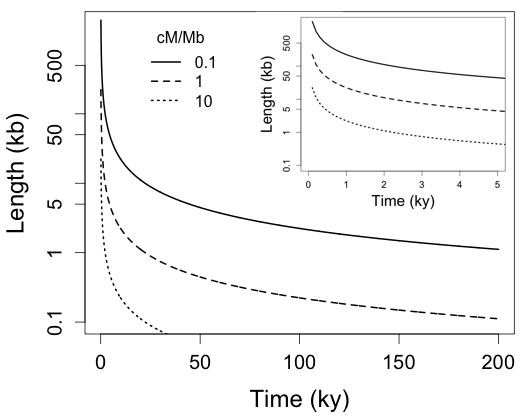
\includegraphics[width=0.6\textwidth]{length_vs_time2}
    \caption{Effect of recombination on the expected length of a shared chromosome segment vs. number of years since divergence or introgression.  Shown are three levels of recombination roughly representing high, average, and low recombination regions of the maize genome.} 
\label{fig:length}
\end{SCfigure}

\subsubsection{Can a widespread species serve as a bridge for introgression among allopatric species?}
\label{sss:bridge}

Our initial survey of divergence and gene flow in \emph{Zea}, based on a set of 26 Sanger-sequenced loci, found evidence for admixture between allopatric populations of \emph{mexicana} and \emph{luxurians} at multiple loci \citep{Ross-Ibarra2009a}. 
As there is no evidence to suggest that these populations overlapped in their recent history, we took these results to suggest that maize, which is known to hybridize with both taxa, may have served as a bridge for gene flow between them.
Further support for this idea comes from patterns of haplotype segregation at an inversion locus on chromosome 4 \citep[\emph{Inv4m};][]{Fang2012,Pyhajarvi2013,Hufford2013}. 
The inverted haplotype at this locus appears to be derived in \emph{mexicana} \citep{Pyhajarvi2013}, but has introgressed into maize in the highlands of Mexico, an apparent example of adaptive introgression \citep[Panel A, Figure \ref{fig:hufmap};][]{Hufford2013}.
We have screened the $>2000$ samples in this data set for a SNP diagnostic for the inverted \emph{mexicana} haplotype and have found that the \emph{mexicana} haplotype is segregating in maize in the highlands of both Mexico and Guatemala (Panel B, Figure \ref{fig:hufmap}).  The haplotype is also present in all samples of \emph{luxurians} genotyped in \citet{Fang2012}.
These preliminary results suggest that the inversion has moved from \emph{mexicana} into \emph{luxurians}, perhaps via a maize intermediate.

\begin{figure}[]
  \centering
   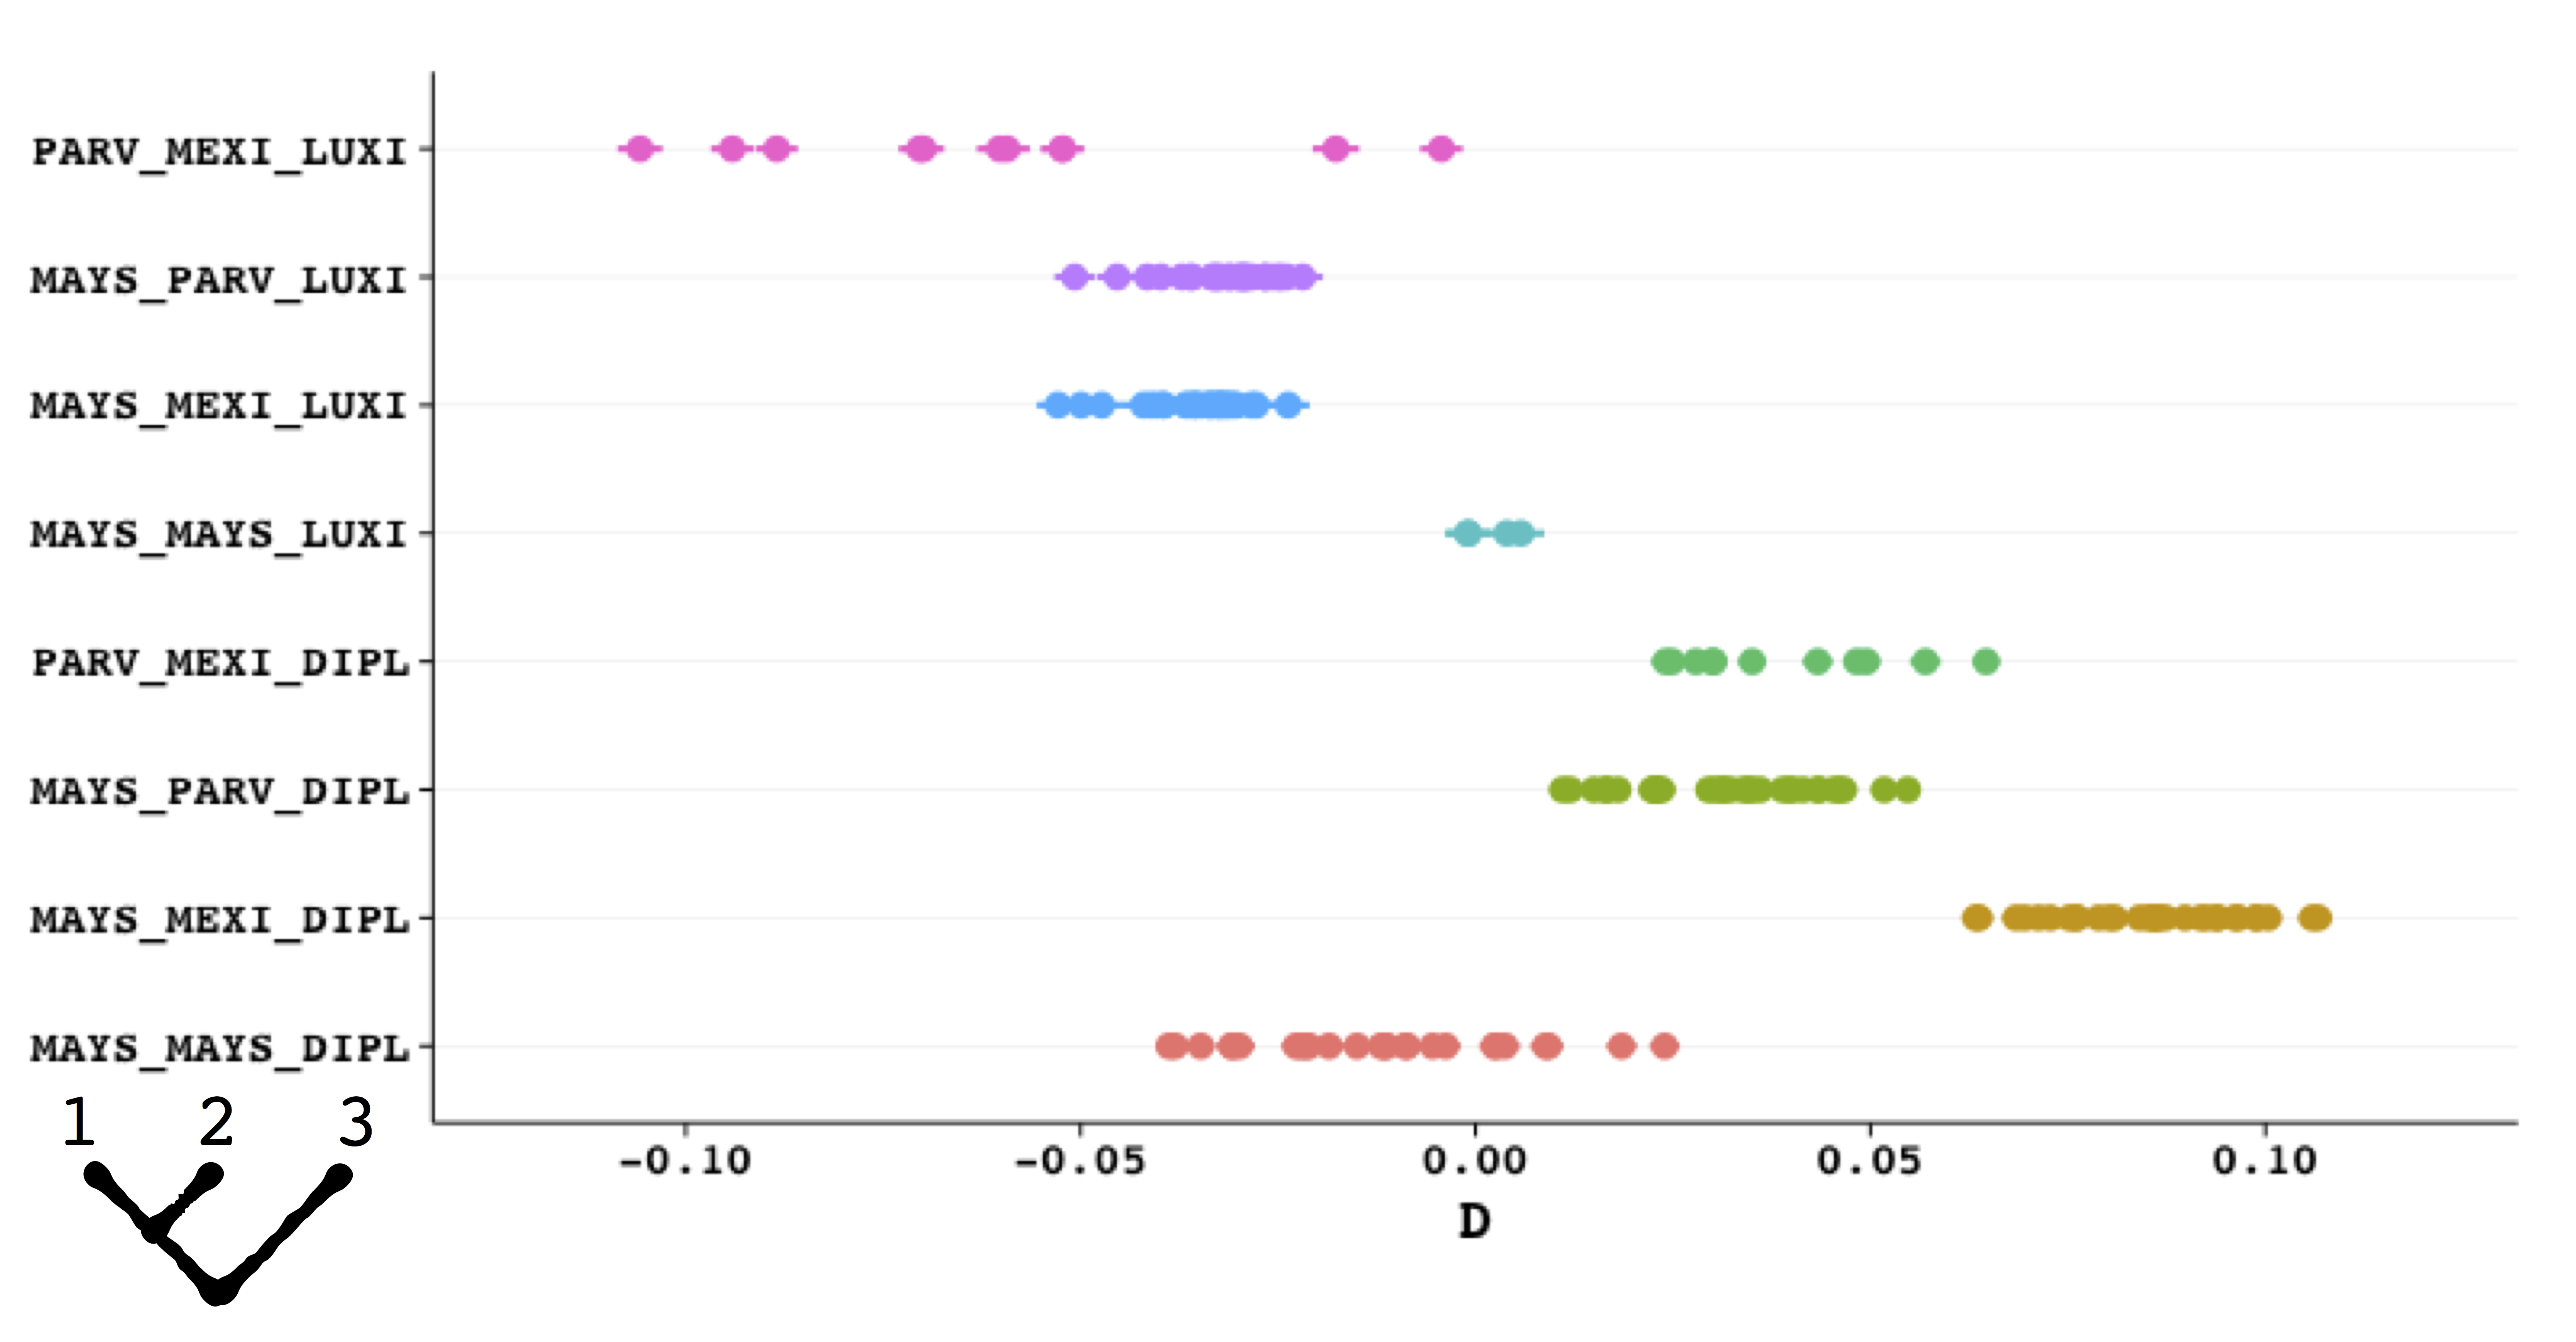
\includegraphics[width=0.8\textwidth]{abbas}
    \caption{Genome-wide evidence for admixture among \emph{Zea}. In the absence of admixture, taxa 1 and 2 on the tree shown should share similar numbers of derived alleles with taxa 3 due to incomplete lineage sorting.  Admixture leads to deviations from this expectation as measured by the D statistic  \citep{green2010draft}. Negative values of D indicate admixture between taxa 1 and 3, while positive values indicate admixture between taxa 2 and 3.} 
\label{fig:abba}
\end{figure}

%\begin{figure}[h!]
%  \centering
%   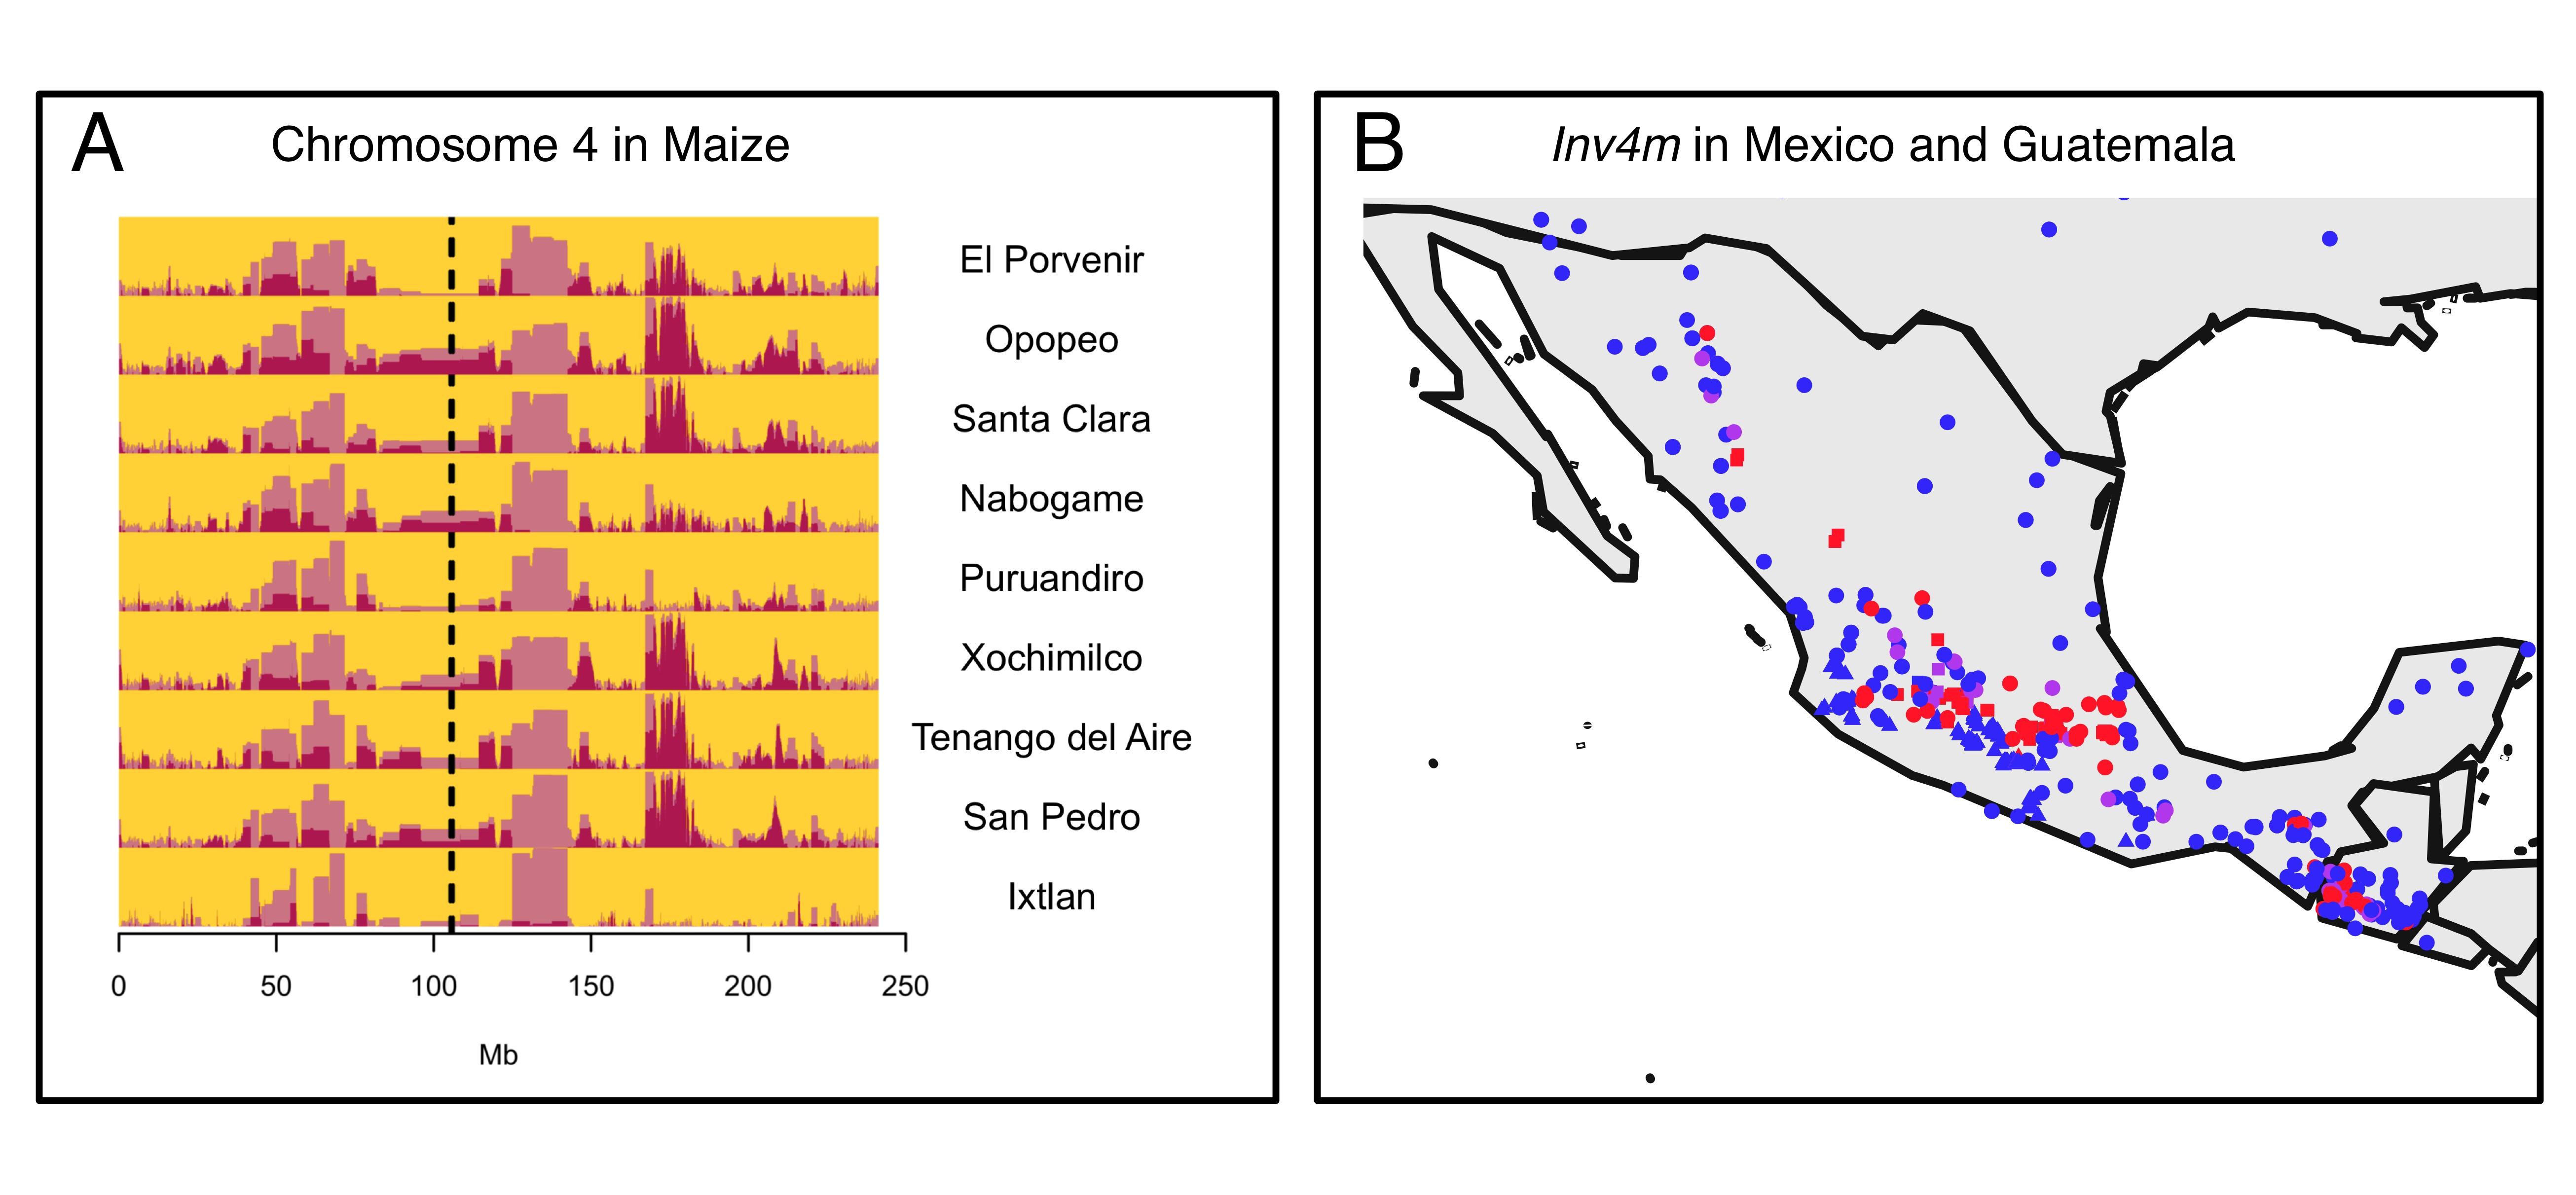
\includegraphics[width=1\textwidth]{inv_map.jpg}
%    \caption{A) Introgression from \zm\ to maize along chromosome 4.  Each row represents a population of maize, and the proportion of individuals with a \zm\ allele at a given position along the genome is shown in dark red.  Light red represents chromosomal regions identified as having a high false positive rate in null permutations.  The strong signal of introgression at Mb 170 is the inversion polymorphism \emph{Inv4m}. B) Geographic distribution of alleles at a SNP found to be diagnostic of the \emph{Inv4m} inversion.  Genotypes are shown in color (blue: homozygous standard, purple: heterozygous, red: homozygous inverted) and shapes represent taxa (squares: \zm, triangles: \zp, circles: domesticated maize)} 
%\label{fig:hufmap}
%\end{figure}


Our preliminary analyses identified shared haplotypes in allopatric teosinte taxa, suggesting that maize may have served as a bridge for gene flow between \emph{mexicana} and \emph{luxurians} and potentially other \emph{Zea} taxa (see above).  However, an alternative explanation is that these loci were polymorphic in a common ancestor and continue to segregate due to incomplete lineage sorting.
Simple estimates of the length of shared haplotypes expected to be unbroken by recombination suggest that, over the $\sim 140,000$-generation divergence time between \emph{mexicana} and \emph{luxurians} \citep{Ross-Ibarra2009a}, we might well expect to see shared haplotypes of even several kb in length in low recombination regions of the genome (Figure \ref{fig:length}).
The high-density, genome-wide data generated here will provide an opportunity to test whether observed patterns of haplotype sharing between previously allopatric \emph{Zea} are due to recent introgression from maize.  
If shared haplotypes have come from introgression from maize over the last few thousand years, the genome-wide distribution of shared haplotype lengths should reveal longer shared segments (Figure \ref{fig:length}) than if haplotype sharing is due to incomplete lineage sorting alone.

No high-resolution genetic map currently exists for any teosinte, but the Ross-Ibarra group is currently working on producing such a map for \emph{parviglumis} as part of a different NSF project (\# 1238014), and evidence from comparisons among maize populations finds remarkable stability of the genetic map at a relatively coarse scale \citep{bauer2013} suggesting differences in the genetic map are unlikely to dramatically affect our estimates. 
Will will use our teosinte genetic map or the published NAM map \citep{McMullen2009} to generate an expected distribution of shared haplotype lengths along the genome based on expected divergence times between taxa.

Although the limited sampling in \citet{Ross-Ibarra2009a} only identified shared haplotypes between \zm\ and \zl, maize has been found to hybridize with all species in \emph{Zea} \citep{Wilkes1977}.
We will thus include in our analysis here the perennial taxa \emph{Zea diploperennis} (hereafter, \emph{diploperennis}) and \emph{Zea perennis} (hereafter, \emph{perennis}).  
We will sample 12 individuals from each of two populations of \emph{diploperennis} and \emph{perennis} and genotype these using GBS.
These populations, combined with samples from other teosinte populations included in \ref{sss:adaptive_intro} and \ref{sss:scale}, will provide us with a representative sample of wild teosinte populations from across the Americas.
Shared haplotypes will be identified (see methods in \ref{sss:genomescan}) and compared to the expected distribution of haplotype lengths to look for evidence of recent introgression consistent with the hypothesis that maize has served as a bridge for gene flow among teosinte taxa.
Although we cannot exhaustively test for the presence of such haplotypes in all of maize, we can survey published GBS data for more than $>16,000$ maize samples (\url{www.panzea.org}) to assess the frequency of such haplotypes in domesticated maize.

\subsubsection{Preliminary Results}
We have made arrangements with collaborators to assist in collection of maize, \zl\ and \zh\ from Guatemala.  The Ross-Ibarra and Hufford labs already have sufficient seed for all other samples for \ref{sss:bridge} and \ref{sss:scale}.
\jri{need more here}

\subsubsection{Potential Challenges}
\jri{need more here}


\section*{Broader Impacts}

Our efforts to broaden the impact of the research proposed here will begin within our groups through our commitment to effectively mentor volunteer undergraduate interns as well as graduate students and/or postdoctoral scholars funded by the project. Students and postdocs will receive one-on-one training from the investigators and senior personnel on laboratory, computational, and field research methods.  Mentees will also be encouraged and funded to present their work at scientific conferences.  Our groups have an excellent mentoring track record with four undergraduate students in the last five years publishing their work in scholarly journals and multiple underrepresented minorities participating in our research.

\jri{add something about undergraduate researchers in my lab?}

%\subsection*{ISU GK12 Fellowship Program}
%	
%In addition to the student and postdoc mentoring that will occur within our groups, as part of our broader impact activities each year one of our graduate students will participate in Iowa State University's GK12 Fellowship program (\emph{Symbi}; \url{http://www.gk12.iastate.edu/default.asp}; see attached letter of commitment). The selected graduate student will spend one full day each week in a middle or high school science classroom for the entire academic year of the Des Moines Public School District. This is the largest and most diverse school district in Iowa with over 50\% underrepresented minority student enrollment and over 70\% of students receiving free or reduced-cost lunch. The graduate student will introduce the K12 students to the scientific process through inquiry-based activities, relate the students’ science curriculum to real world examples, work with students on their science fair projects, and serve as a role model in a STEM profession. Furthermore, the graduate student will introduce students to his/her research project on hybridization and introgression in \emph{Zea}, a topic that is particularly well suited for teaching evolution in Iowa given the important role that maize plays in the Iowan economy. In introducing his/her dissertation research, the graduate student will engage Des Moines students in how research is conducted and provide STEM content professional training to his/her partner teacher.
%
%The GK12 Fellow will work with approximately 150 students on a regular weekly basis.  Student assessments from the ISU GK12 Fellowship Program have shown that a significant number of students like science more after having a GK Fellow in the classroom.  Teachers report that having a GK12 Fellow in their classroom is excellent professional development.  The PI will also visit the classroom and will support the selected graduate student in their development of appropriate material for the K12 audience.

\subsection*{US-Mexico Exchange Program}
	
Finally, we will establish a student exchange program between the Eguiarte Laboratory at UNAM in Mexico and the Hufford and Ross-Ibarra Laboratories in the United States. The Ross-Ibarra Laboratory has run an NSF-supported, US-Mexico exchange program for the last four years.  All of the exchange students involved in the program have continued on to additional graduate work, and two have earned authorship on forthcoming papers from their internship.  We will build upon the success of this program.  A student from the Eguiarte group will spend 2-3 months in either the Hufford or Ross-Ibarra Laboratory learning the GBS methodology and/or honing his/her skills in population genomic analysis, whereas a student from the Hufford and/or Ross-Ibarra Laboratories will travel to Mexico to participate in sample collection trips and to obtain expertise in common garden field experiments. This exchange will build capacity in all groups involved and will provide a valuable international research experience for a graduate student supported by the grant.  

Senior Personnel Claudia Calder\'{o}n has previously led international student research trips and will assist in preparing students from both the United States and Mexico for the exchange program. A survey will be given to both exchange students and faculty in order to gauge expectations prior to the trip and facilitate collaborations amongst the labs.  The survey will also assess students' knowledge and preconceived ideas  regarding their travel destinations.  A meeting (online or face-to-face) with the cohort of students traveling will help address these pre-conceptions and reduce cultural misunderstandings.  Suggestions will be given to students of how to prepare before the trip (visa, immigration requirements) and how to communicate with their peers and others during their exchange.  Students will be given information regarding the facilities where they will be staying, transportation to be used, food and water safety, the availability of telecommunications and general safety guidelines.

\required{Results From Prior NSF Support}
% 5 pages or fewer of the 15 pages for entire description document.
% include results from NSF grants received in the past 5 years.
% If supported by more than one grant, choose the most relevant one.

% For each grant, include: 
%	(a) NSF award number, amount, dates of support 
%	(b) The title of this project
%	(c) Publications resulting from this research
%	(d) Summary of the results of the completed work
%	(e) A brief description of data samples available and other research products not described 	      elsewhere
%	(f) For renewed support, a description of the relationship between the completed and 			      proposed work

% Due to space limitations, it is often advisable to use citations rather
% than putting the titles of the publications in the body 
% of this section

\subsection*{Hufford, Ross-Ibarra, Coop, Flint-Garcia, Sawers: \#1404974: US-Mexico Planning Visit and Workshop to Assess the Genomic Basis of Local Adaptation in Maize}
\$34,650. 09/01/14-08/31/15. PI Matthew Hufford, co-PIs J. Ross-Ibarra, G. Coop, Senior Personnel S. Flint-Garcia, Collaborators R. Sawers and A. Cibrian-Jaramillo
\par\noindent{\bf Intellectual merit} Through planning meetings and a phenotyping workshop in Mexico, this project has established a new international collaboration amongst principal investigators and laid the foundation for the work proposed in the current Plant Genome Research Program proposal. Planning meetings helped coordinate generation of preliminary data described in this proposal and the phenotyping workshop transferred high-throughput methods across our research groups.
\par\noindent{\bf Broader impacts}  Participants in the phenotyping workshop included graduate students and postdoctoral scholars from the United States and Mexico, providing STEM training and an international scientific experience.
\par\noindent{\bf Publications} Funding is for organizational purposes and generation of preliminary data; no publications have been produced under this award.

%\subsection*{Ross-Ibarra: \#1238014: Biology of Rare Alleles in Maize and Its Wild Relatives}
%\$13,311,185 (\$2,368,767 to Ross-Ibarra), 05/15/13-04/30/18. PI Edward Buckler, co-PIs J. Doebley, J. Holland, S. Flint-Garcia, Q. Sun, P. Bradbury, S. Mitchell, J. Ross-Ibarra
%\par\noindent{\bf Intellectual merit} In the first year we have developed accurate imputation approaches, found evidence for the importance of deleterious variants and non-genic polymorphisms in heterosis and GWAS, documented differences in recombination among the parents of the NAM population, and found population genetic evidence suggesting the importance of demography and purifying selection across the genome.  The grant has produced 18 total publications in its first year (only publications involving PIs Flint-Garcia and Ross-Ibarra are shown below).
%\par\noindent{\bf Broader impacts}  In the first year this project has included 10 postdoctoral and 12 graduate trainees. The GBS workshop and traveling maize exhibit continue to be popular and successful. A new version of the teacher-friendly guide to maize evolution has been revised and published online.
%\par\noindent{\bf Publications} \citet{peiffer2013genetic, Romay2013, wills2013many, Mezmouk2014, Peiffer2014, sood2014mining}

\subsection*{Ross-Ibarra: \#0922703: Functional Genomics of Maize Centromeres}
\$5,008,031 (\$754,409 to Ross-Ibarra). 09/01/09-08/31/14. PI Kelly Dawe, co-PIs J. Birchler, J. Jiang, G. Presting, J. Birchler, J. Ross-Ibarra
\par\noindent{\bf Intellectual merit} Centromeres are regions of the genome that organize and regulate chromosome movement, yet the biology of centromeres remains poorly understood. Co-PI Ross-Ibarra's group has focused in particular on the evolutionary genetics of centromeres. This work has demonstrated the remarkable evolutionary lability of centromere tandem repeats, but has shown that there is little evidence in maize for coevolution between centromere sequence and kinetochore proteins. Ongoing work from the Ross-Ibarra lab seeks to characterize kinetochore proteins, assess the phylogenetic evidence for longer-term coevolution, and understand patterns of centromere and genome size variation in natural populations.
\par\noindent{\bf Broader impacts}  Co-PI Ross-Ibarra has established an international student exchange program as part of this grant. Data and results of this project have been disseminated via publications and presentations as well as deposited in the maize genetics community database \url{www.maizegdb.org}. Former trainees on the grant include Dr. Matthew Hufford (PI on the current grant).\
\par\noindent{\bf Publications} \citet{Shi2010a, Chia2012a, Fang2012, Hufford2012, Hufford2012b, Hufford2013, Melters2013a, Kanizay2013, Pyhajarvi2013}% 
%%%%%%%%%%%%% References no page limit %%%%%%%%%%%%%%%%%%%
\setcounter{page}{1}
%%%%%%%%% References Cited

%	Reference information is required. 

%	Each reference must include the names of all authors (in the same sequence in which they appear in the publication), the article and journal title, book title, volume number, page numbers, and year of publication. 

%	If the document is available electronically, the website address also should be identified. 

%	Proposers must be especially careful to follow accepted scholarly practices in providing 			citations for source materials relied upon when preparing any section of the proposal. 

%	While there is no established page limitation for the references, this section must include bibliographic citations only and must not be used to provide parenthetical information outside of the 15-page project description.

%	For Example : 

%	\begin{thebibliography}{99}
%	\bibitem{paper01} Name, {\em Title of the article}, Journal the article appears in, Year(YYYY).
%	\end{thebibliography}
	

% In case of including a BibTeX or .bib file, use the following command :

%\bibliographystyle{apalike}
\bibliography{references}
%%%%%%%%%%%%% Biosketch  Max two pages per person%%%%%%%%%%%%%%%%%%%
%\setcounter{page}{1}
%%%%%%%%%% BIOGRAPHICAL SKETCH --  Maximum 2 pages 

\required{Biographical Sketch: Your Name}
\begin{center}
\emph{Maximum of 2 pages}
\end{center}•

% Your Bio should be divided into the following sections

%	I.	Professional Preparation
%		------------------------------------------

%	*	Mention a complete list of undergraduate and graduate education and postdoctoral 		                     training as shown:

%		Institution(s)			Major			Degree		Year
%		------------------- 			--------- 			------------ 		-------
%		Undergraduate
%		Graduate
%		Postdoctoral			(Area)			N/A
%		-------------------------------------------------------------------------------------------------------

\setcounter{page}{1}
\renewcommand{\thepage}{Biographical Sketch - Page \arabic{page} of 2}
\begin{center}
\textbf{\large Biographical Sketch}
\end{center}

{\bf Professional Preparation}

\begin{tabular}{llll}
Undergraduate Institution(s) \hspace{0.5in} & Major \hspace{1in} & Degree  \hspace{0.25in} & Year \\
Graduate Institution(s)                     & Major              & Degree                  & Year \\
Postdoctoral Institution(s)                 & Area               &                         & Year
\end{tabular}

%	II.	Appointments
%		------------------------

%	*	A list in reverse chronological order of all academic / professional appointments
%		beginning with the current appointment as shown:

%		------------------------------------------------------------------------
%		Year(s)	Position, Department, Institution
%		------------------------------------------------------------------------

\begin{tabular}{ll}
Year-present & Position, Department, Institution \\
Year(s)      & Position, Department, Institution \\
\end{tabular}

%	III. 	Publications
%		---------------------

%	*	Up to 5 publicationa most closely related with the porposed project
%	*	Up to 5 other publications, whether or not related to the proposed project
%	* 	Each publication must include the names of all authors in the same sequence as they
%		appear in the publication, the article and journal title, book title, volume number, page
%		numbers and year of publication.
%	*	The website address should be included if the document is available electronically
%	*	List any unpublished manuscripts that have been accepted for publication; also include
%		the most likely date of publication.
%	* 	Patents, copyrights and software systems may be substituted for publications.
%	*	Only the list of 10 publications will be used in the review of the proposal.

\vspace{12pt}
{\bf  Publications}

\vspace{12pt}
\emph{Five Publications Most Closely Related to the Proposed Project}

\begin{enumerate}
\item Author(s): Article Title, \emph{Journal Title} {\bf Volume Number}, Page Numbers, Year of Publication.

\item

\item

\item

\item
\end{enumerate}

\vspace{12pt}
\emph{Ten Other Significant Publications}

\begin{enumerate}
\item

\item

\item

\item

\item

\item

\item

\item

\item

\item
\end{enumerate}

%	IV.	Synergistic Activities
%		-----------------------------------

%	*	List up to five examples that demonstrate the broader impact of the professional 
%		and scholarly activities that focuses on the integration and knowledge transfer as 
%		well as its creation.
%	*	Examples could
%		include, among others: innovations in teaching and training (e.g., development
%		of curricular materials and pedagogical methods); contributions to the science
%		of learning; development and/or refinement of research tools; computation
%		methodologies, and algorithms for problem-solving; development of databases
%		to support research and education; broadening the participation of groups
%		under-represented in science, mathematics, engineering and technology; and
%		service to the scientific and engineering community outside of the
%		immediate organization.
\begin{enumerate}
\item

\item

\item

\item

\item
\end{enumerate}

\vspace{12pt}
{\bf Collaborators \& Other Affiliations}

\vspace{12pt}
\emph{Collaborators:}
%A list of all persons in alphabetical order (including their current
%organizational affiliations) who are currently, or who have been collaborators
%or co-authors on a project, book, article, report, abstract
%or paper during the 48 months preceding the submission of this proposal.
%Also include those individuals who are currently or have been co-editors
%of a journal, compendium, or conference proceedings during the 24 months
%preceding the submission of the proposal. If there are no collaborators
%or co-editors to report, this should be so indicated.

\vspace{12pt}
\emph{Graduate and Postdoctoral Advisors:}
%A list of the names of the individual's own graduate advisor(s) and
%principal postdoctoral sponsor(s), and their current organizational
%affiliations.

\vspace{12pt}
\emph{Thesis Advisor and Postgraduate-Scholar Sponsor:}
%A list of all persons (including their organizational affiliations),
%with whom you have had an association as thesis advisor, or with
%whom your have had an association within the last five years as a
%postgraduate-scholar sponsor. The total number of graduate students advised
%and postdoctoral scholars sponsored also must be identified.
%%%%%%%%%%%%% Budget Justification  no more than 3 pages %%%%%%%%%%%%%%%%%%%
%\setcounter{page}{1}
%\renewcommand{\thepage}{f. Budget Justification - Page \arabic{page} of 3}

\required{Budget Justification}
%\begin{center}
%\emph{Maximum of 3 pages}
%\end{center}

\subsection*{Personnel}

No funding is requested for the PI, Co-PIs, or any Senior Personnel.

\subsection*{Other Personnel}
\paragraph{Graduate students} 
Funds are requested to support two graduate students each for 6 months during the academic year for each year of the project. At UC Davis, the current pay rate for doctoral students at 50\% FTE is \$27,319 during the academic year. Included is the estimated annual salary increase of 3\%.  The two students will be working on analysis of GBS data in the introgression and admix population genetic sections of \ref{sec:popgen}, and will likely help with QTL analysis and sequencing in \ref{sec:qtl}, and potentially RNA-seq analysis in \ref{sec:funchar}.

\paragraph{Technician}
Funds are requested for the first three years of the grant for a 50\%-time technician (Laboratory Assistant III) to extract DNA and RNA, prepare genomic and transcriptomic sequencing libraries, and perform root chilling experiments.  The salary for this positions is set at \$36,000 (\$18,000 for 50\% time), with an annual increase of 5\%.

\subsection*{Fringe Benefits}
Fringe benefits are applied to personnel salaries using the university approved rates:
\begin{itemize}
%\item Faculty - \% in FYs 2012, 2013, and 2014
%\item Postdocs - \% in FYs 2012, 2013, and 2014
\item Graduate students - 1.3\% for all years.
%\item Undergraduate students - \% in FYs 2012, 2013, and 2014
\item Technician - 50.4\%(1/1/2015-6/31/2015), 53.4\%(6/31/2015-6/31/2016), 55.7\%(6/31/2016-6/31/2017), 57.3\%(6/31/2017-12/31/2017)
%\item Part time staff - \% in FYs 2012, 2013, and 2014
\end{itemize}

\subsection*{Equipment}

No equipment funds are requested.

\subsection*{Travel}

Travel for the PI and Co-PI Coop and one student to 1 domestic conference each year is budgeted at \$3,000.  Travel for one of the Senior Personnel or Co-PIs to participate in the field workshop is budgeted at \$1,000 each year.

Travel for Senior Personnel and members of their group to manage field experiments and phenotype is budgeted at \$12,000 each of the first 3 years. Travel for both Senior Personnel to 1 international conference each year is budgeted at \$3,000 per year.

\subsection*{Participant Support}
Our exchange program proposes to exchange two students per year between the US and Mexico.  We are requesting funds to pay for 2 exchange students per year of the grant. These funds will cover student subsistence (\$1,800 a month to include housing and subsistence) for 3 months, visa costs (\$500), and round-trip travel to Mexico (\$2,000).

\subsection*{Other Direct Costs}

 \paragraph{Materials and Supplies}
In each of the first three years of the grant, \$15,000 is requested in materials and supplies.  \$10,000 of this is for laboratory supplies for PI Ross-Ibarra for library prep for whole genome sequencing, RNA sequencing, and DNA extraction and preparation for GBS.  This also includes funds for supplies for root chilling experiments to be done at UC Davis.  In each of the five years, \$2,500 is budgeted for standard office supplies, computer supplies (extra storage for our cluster, backup drives for lab members), and other miscellaneous expenses for Co-PI Coop and PI Ross-Ibarra. 

\paragraph{Whole genome sequencing}
The genomes of each of the four parental lines of our QTL mapping populations will be resequenced to a depth of 20-30X using 2 lanes of paired end 150bp reads on an Illumina HiSeq 2500. Current lane costs are approximately \$2,200 per lane, and library preparations costs are approximately \$100, for a total cost of \$18,000.

\paragraph{GBS}
Genotyping-by-sequencing will be performed for our introgression and admixture population genetic analyses. GBS will be performed at the Institute for Genomic Diversity at Cornell.  Current prices are \$60 per sample to run samples at 48-plex.  We will genotype 360 individuals for our introgression analysis in year 1 for a cost of \$21,600, and 144 individuals in year 2 for a cost of \$8,640. 

\paragraph{RNA sequencing}
In total, RNA sequencing will be performed on 384 individuals (8 inbreds x 2 stages x 2 tissues x 2 environments x 3 replicates + 8 NILs x 2 genotypes x 2 stages x 2 environs x 3 replicates).  Cost to prepare RNA libraries in our lab are approximately \$100 per library, and sequencing costs for single-end 50bp reads at the UCD Genome Center are approximately \$1,000 per lane.  Multiplexing 12 barcodes per lane, this comes out to 32 lanes of sequence and a total cost of \$70,400.

\paragraph{Field fees}
Fees for the field experiments in our highland and lowland field sites (Table \ref{tab:locales}) are approximately \$60,000 the first three years of the experiment to allow development of the mapping populations and two replicates of the phenotyping.  These fees include land rental and basic management (planting, watering, weeding, fertilizing), as well as station fees to hire manual labor for phenotyping.  These fees decrease to \$10,000 in the last two years of the proposal as subsequent field experiments including evaluation of NILs and RNA-seq lines, will be considerably smaller. Field fees total \$200,000 across the five years of the grant.

\paragraph{Graduate Student Tuition}
Tuition for graduate students is charged to the project in proportion to the amount of effort the graduate student will work on the project. For a graduate student employed on the project for 9 academic months at 50\% FTE, the tuition charge is \$31,546 in FY 2015 to account for out-of-state tuition, \$17,266 in FY 2016 and increasing 5\% each subsequent year.

\paragraph{Publication Costs}
In year two \$1,500 is requested for publication fees to an open access journal.  In subsequent years \$3,000 is requested annually.

\subsection*{Total Direct Costs}

Total direct costs for UCD come to \$874,643.  Subawards to USDA-ARS and Iowa State total \$1,218,560.

\subsection*{Indirect Costs}
Indirect costs are calculated on Modified Total Direct Costs (Total Direct costs less graduate student fees and participant support and subaward funding beyond the first \$25,000) using F\&A rates approved by US Department of Health and Human Services. For this project, F\&A rates of 55.5\% were used from Jan. 1, 2015 through June 30, 2015, 56.5\% from July 1, 2015 through June 30, 2016, and 57\% from July 1, 2016 until the end of the project.% 
%%%%%%%%%%%%% Facilities Max 1 page %%%%%%%%%%%%%%%%%%%
\setcounter{page}{1}
\required{Facilities, Equipment, and Other Resources}

\setcounter{page}{1}
\renewcommand{\thepage}{Facilities, Equipment, and Other Resources - Page \arabic{page} of 2}

%\begin{center}
%\textbf{\large Facilities, Equipment \& Other Resources}
%\end{center}

%	Identify the facilities to be used, as appropriate, indicate their capacities,
%	pertinent capabilities, relative proximity, and extent of availability to the project.
%	Use ``Other" to describe the facilities at any other performance sites listed and at
%	sites for field studies.

% \textbf{Laboratory:}
% 
% \textbf{Clinical:}
% 
% \textbf{Animal:}

%\textbf{Computer:}

%	List in detail the computing capabilities of the university and the department

%\textbf{Office:}

%\textbf{Other:}

%\textbf{MAJOR EQUIPMENT:}

%	List the most important items available for this project and, as appropriate
%	identifying the location and pertinent capabilities of each.

%\textbf{OTHER RESOURCES:}

%	Provide any information describing the other resources available for the
%	project. Identify support services such as consultant, secretarial,
%	machine shop, and electronics shop, and the extent to which they will be
%	available for the project. Include an explanation of any consortium/
%	contractual arrangements with other organizations.

\paragraph{\textbf{Iowa State University}}\

Project components completed in the Hufford Laboratory at Iowa State University (ISU) will include DNA isolation and preparation for genotyping and population genetic analysis of genotyping and full-genome sequence data. The Hufford Laboratory has all equipment necessary for DNA isolations, quality control and preparation for genotyping including centrifuges, thermal cyclers, an ultra-low freezer, water baths, a pH meter, balances, and an electrophoresis system. A gel imaging system and a NanoDrop spectrophotometer for DNA quantification are accessible through the Center for Plant Responses to Environmental Stresses at ISU. Genotyping will be carried out using a reduced representation approach to next-generation sequencing known as Genotyping by Sequencing (GBS) at the Genomic Diversity Facility at Cornell University (see letter of commitment from Sharon Mitchell). Full-genome sequencing will be carried out at the DNA Facility at ISU, which provides access to cutting-edge genomic technologies including HiSeq and MiSeq Illumina sequencing and library preparation for both paired-end and mate-pair approaches. Data analyses will be carried out using the High Performance Computing clusters available at ISU. Dr. Hufford currently has access to the Lightning3 cluster which has a mix of Opteron based servers, consisting of 18 SuperMicro servers with core counts ranging from 32 to 64 and 256 to 512 GB of memory.  Broader impacts at ISU will be facilitated by the \emph{Symbi} program. \emph{Symbi} was Iowa's first GK12 program and represents a partnership between the Des Moines Public School System and Iowa State University.  Staff members from \emph{Symbi} have experience facilitating over 30 previous graduate student fellows in communicating their science to grade school students and will assist the graduate student funded by this project to do the same (see letter of commitment from \emph{Symbi}).

\paragraph{\textbf{UC Davis}}\

Dr. Ross-Ibarra has four standard laboratory benches as part of a shared lab space at UCD.  The shared space is the single largest lab space on campus, and provides for seamless interaction between the labs housed there.  The space currently houses three other PIs, all working on the genetics and genomics of economically important plant taxa (Dubcovsky, Neale, Dandekar). The lab is equipped with standard equipment and tools for molecular biology, including freezers and refrigeration, a shared liquid handling robot, thermal cyclers, centrifuges, gel rigs, balances, and standard molecular biology supplies.  A dedicated low-humidity refrigerator for seed storage is available through the university, and low-humidity storage cabinets for tissues and temporary seed storage are in the laboratory. Dr. Ross-Ibarra occupies half of a large office suite that includes a conference room and cubicle space for 25 people.  Both Macintosh and PC workstations are available for student and postdoc employees. Dr. Ross-Ibarra is a contributing partner in a large computer cluster, giving the lab dedicated access to 192 processors, with the opportunity for use of nearly 800 additional CPU as resources allow. Recent (2013) additions to the cluster have provided it with additional CPU as well as six new shared high-memory (512Gb RAM) nodes, one of which is dedicated to the Ross-Ibarra lab. Dr. Ross-Ibarra is a faculty member of the UC Davis Genome Center, a large facility that includes bioinformatics, genotyping, metabolomics, proteomics, and expression analysis cores able to perform a variety of genomics analyses at cost for UC Davis faculty. The Genome Center also rents time on its equipment, including a bioanlyzer and library preparation robots. As a member of the Genome Center, Dr. Ross-Ibarra also has access to their additional computational facilities. UC Davis has also entered into a recent partnership with BGI (formerly the Beijing Genomics Institute) to provide additional high-throughput sequencing services via a new Sacramento-based sequencing facility.

\paragraph{\textbf{Partners in Mexico and Guatemala}}\

Senior Personnel on this project include Luis Eguiarte of UNAM in Mexico City and Claudia Calder\'{o}n, a Guatemalan national.  This project will benefit greatly from their many years of experience working in the field in Mexico and Guatemala respectively.  In addition we have confirmed commitments from Ruairidh Sawers of Langebio in Irapuato, Mexico and Salvador Montes-Hernandez of Inifap in Celaya, Mexico (see attached commitment letters) to assist with common garden experiments.  Between Dr. Sawers and Dr. Montes-Hernandez, our collaborators have ample experience growing maize and teosinte in nurseries located on the West Coast (Valle de Banderas, Nayarit), in Central Mexico (Irapuato and Celaya, Guanajuato), and in the high valleys of Central Mexico (Queretero, Estado de Mexico). They also regularly conduct field expeditions to collect plants in both the dry regions of Northern Mexico (maize collections in Chihuahua, Lamiaceae throughout the Northeast) and the lower valleys of the Eje Volcanico and Costa del Pacifico (teosinte and maize, Solanaceae, and Cucurbitaceae).  A commitment has also been confirmed (see attached letter) from Mario Fuentes L\'{o}pez to assist with teosinte collection in Guatemala.
\clearpage
\newpage
% Supplementary Documents
%%%%%%%%%%%%% Data Management 1 page REQUIRED
\setcounter{page}{1}
\setcounter{page}{1}
\renewcommand{\thepage}{Data Management Plan - Page \arabic{page} of 2}
%\required{Supplementary Documentation}
\required{Data Management Plan}
%\begin{center}
%\emph{Maximum of 2 pages}
%\end{center}•
% Maximum of 2 pages
%------------------------------

% This supplement should describe how the proposal will conform to NSF policy on
% the dissemination and sharing of research results and may include:
% 
% 1. The types of data, samples, physical collections, software, curriculum
%    materials, and other materials to be produced in the course of the project;
% 
% 2. The standards to be used for data and metadata format and content (where
%    existing standards are absent or deemed inadequate, this should be documented
%    along with any proposed solutions or remedies);
% 
% 3. Policies for access and sharing including provisions for appropriate
% protection   of privacy, confidentiality, security, intellectual property, or
% other rights or   requirements;
% 
% 4. Policies and provisions for re-use, re-distribution, and the production of
%    derivatives; and
% 
% 5. Plans for archiving data, samples, and other research products, and for
%    preservation of access to them.
% 
% A valid Data Management Plan may include only the statement that no detailed
% plan is needed, as long as the statement is accompanied by a clear
% justification. Proposers who feel that the plan cannot fit within the supplement
% limit of two pages may use part of the 15-page Project Description for
% additional data management information. Proposers are advised that the Data
% Management Plan may not be used to circumvent the 15-page Project Description
% limitation.

%(A-1) Sharing of Results and Management of Intellectual Property (maximum 3 pages): Describe the management of intellectual property rights related to the proposed project, including plans for sharing data, information, and materials resulting from the award. This plan must be specific about the nature of the results to be shared, the timing and means of release, and any constraints on release. The proposed plan must take into consideration the following conditions where applicable:
%
%Sequences resulting from high-throughput large-scale sequencing projects (low pass whole genome sequencing, BAC end sequencing, ESTs, full-length cDNA sequencing, etc.) must be released according to the currently accepted community standard (e.g. Bermuda/Ft. Lauderdale agreement) to public databases (GenBank if applicable), as soon as they are assembled and quality checked against a stated, pre-determined quality standard. "At publication" is not acceptable.
%Proposals that would develop genome-scale expression data through approaches such as microarrays or next-generation sequencing should meet community standards for these data (for example, Minimum Information About a Microarray Experiment or MIAME standards). The community databases (e.g. Gene Expression Omnibus) into which the data would be deposited, in addition to any project database(s) should be indicated.
%If the proposed project would produce genome-scale data sets generated using proteomics and/or metabolomics approaches, NSF encourages that they be made available as soon as their quality is checked to satisfy the specifications approved prior to funding. The timing of release should be stated clearly in the proposal. The community databases into which the data would be deposited, in addition to any project database(s) should be indicated.
%If the proposed project would produce community resources (biological materials, software, etc.), NSF encourages that they be made available as soon as their quality is checked to satisfy the specifications approved prior to funding. The timing of release should be stated clearly in the proposal. The resources produced must be available to all segments of the scientific community, including industry. A reasonable charge is permissible, but the fee structure must be outlined clearly in the proposal. If accessibility differs between industry and the academic community, the differences must be clearly spelled out. If a Material Transfer Agreement is required for release of project outcomes, the terms must be described in detail.
%When the project involves the use of proprietary data or materials from other sources, the data or materials resulting from NSF funded research must be readily available without any restrictions to the users of such data or materials (no reach-through rights). The terms of any usage agreements should be stated clearly in the proposal.
%Budgeting and planning for short-term and long-term distribution of the project outcomes must be described in the proposal. If a fee is to be charged for distribution of project outcomes, the details should be described clearly in the proposal. Letters of commitment should be provided from databases or stock centers that would distribute project outcomes, including an indication of what activities would be undertaken and funds needed for these activities (if any).
%In case of a multi-institutional proposal, the lead institution is responsible for coordinating and managing the intellectual property resulting from the PGRP award. Institutions participating in multi-institutional projects should formulate a coherent plan for the project prior to submission of the proposal.
%

\subsection*{Data Types}

This proposal will generate genotype and full-genome sequence data, phenotype data, analytical code, germplasm, and publications.

\subsection*{Data Archiving, Plan for Sharing, Public Access Policy}

\paragraph{Genotype and Sequence Data} 
All data will be made publicly available and stored online.  However, prior to public release, all data will be hosted locally.  Drs. Hufford and Ross-Ibarra will maintain a backup of all raw genotyping and sequencing data.  Dr. Hufford has access to 144Tb of free data storage through the College of Liberal Arts and Sciences at Iowa State and Dr. Ross-Ibarra maintains a DROBO distributed backup server (currently $>8$Tb of free space) which is robust to single disk failure. All sequence data (whole genome sequencing, and fastq files from genotyping by sequencing) will be submitted immediately upon completion of data quality control to the NCBI sequence read archive (SRA), along with passport information on each parent. A "hold until publication" embargo will be requested at the SRA. Just prior to publication, genotypes will be made publicly available via the Figshare website (\url{www.figshare.com}), a free public website allowing dissemination and archiving of large datasets. Data will be released in accordance with the Toronto agreement (2009. Nature 461:168-170. \url{www.nature.com/nature/journal/v461/n7261/full/461168a.html}) under the stipulation that no whole-genome analyses be performed until we have published our initial analyses.

\paragraph{Phenotype Data} 
Phenotypic data will be recorded digitally in the field using a high-throughput technique developed by Dr. Sherry Flint-Garcia at USDA and the University of Missouri.  Data will be uploaded at the end of each day into the FieldBook database developed by Dr. Flint-Garcia and immediately backed up at a remote location. Data will be grouped into projects, and each project is associated with a unique digital object identifier (DOI). Phenotypic data will then be uploaded to Figshare, along with appropriate metadata associated with other publications, links to germplasm, SRA experiments, Github code, etc.  Data on Figshare are publicly available and searchable.  We will submit data as soon as we complete quality control, but again with explicit stipulations as to the analyses that the data can be used for prior to our initial publication. All appropriate metadata including plant ID, data collector, field location, etc. will be associated with phenotype data deposited to Figshare. 

\paragraph{Analytical Software and Code} 
Analytical software and code from this project will be hosted on Github, a version-controlled public git repository.  Upon submission of papers all code will be made publicly available.  Drs. Hufford and Ross-Ibarra have already done this extensively (see \url{https://github.com/mbhufford} and \url{https://github.com/rossibarra} and \url{https://github.com/rilab}. Publication of all code will ensure reproducibility of all analyses conducted.  All data and code will be made publicly available via a creative commons CC by 2.0 license \url{http://creativecommons.org/licenses/by/2.0/} allowing free access to reuse, redistribute, and modify, requiring only citation of the license and the original source.

\paragraph{Germplasm} 
Sample accession data will be securely stored in MySQL servers hosted at Iowa State University and the University of California, Davis and backed up on a weekly basis offsite.  International agreements prohibit some of the maize and teosinte germplasm collected in Mexico and Guatemala from being stored and distributed by USDA.  We will, however, deposit small quantities of seed from all our collections with the CIMMYT germplasm bank in Mexico, which provides public access to seed.

\paragraph{Publications} 
All publications resulting from this project will be submitted to one or more preprint servers (e.g. arXiv, bioRxiv, PeerJ) such that they will be publicly available immediately upon submission of the paper for publication.% 
%%%%%%%%% Postdoc Mentoring is required if funding requests postdocs MAX 2 pages?
\setcounter{page}{1}
\renewcommand{\thepage}{Postdoctoral Researcher Mentoring Plan - Page \arabic{page} of 1}
\required{Supplementary Documentation}
\required{Postdoctoral Researcher Mentoring Plan}

%\emph{Maximum of 1 page}
%Each proposal that requests funding to support postdoctoral researchers must include, as a supplementary document, a description of the mentoring activities that will be provided for
%such individuals. In no more than one page, the mentoring plan must describe the
%mentoring that will be provided to all postdoctoral researchers supported by
%the project, irrespective of whether they reside at the submitting organization,
%any subawardee organization, or at any organization participating in a
%simultaneously submitted collaborative project. Proposers are advised that the
%mentoring plan may not be used to circumvent the 15-page project description
%limitation.

%\smallskip
%Examples of mentoring activities include, but are not limited to: career
%counseling; training in preparation of grant proposals, publications and presentations;
%guidance on ways to improve teaching and mentoring skills; guidance on how to
%effectively collaborate with researchers from diverse backgrounds and disciplinary areas;
%and training in responsible professional practices. The proposed mentoring activities
%will be evaluated as part of the merit review process under the broader impacts merit
%review criterion. Proposals that include funding to support postdoctoral researchers
%and do not include the requisite mentoring plan will be returned without review.

%\bigskip
%\textbf{Documentation of collaborative arrangements} of significance to the
%proposal through letters of commitment.

%\smallskip
%Proposers are reminded that, unless required by a specific program solicitation,
%letters of support should not be submitted as they are not a standard component
%of an NSF proposal, and, if included, a reviewer is under no obligation to review
%these materials. Letters of support submitted in response to a program solicitation
%requirement must be unique to the specific proposal submitted and cannot be altered
%without the author's explicit prior approval. NSF may return without review proposals
%that are not consistent with these instructions.

%\bigskip
%\textbf{Documentation regarding research involving the use of human subjects}, hazardous
%materials, vertebrate animals, or endangered species.

The current proposal requests funding for one postdoctoral researchers at UC Davis and one at Iowa State. We also hope additional postdocs may join the group via alternative funding opportunities (fellowships, etc.) and anticipate that postdocs funded on other grants may collaborate to a greater or lesser degree on this project.  Much of our thinking on postdoctoral mentoring comes directly from our own mentorship experience -- PIs Hufford and Ross-Ibarra were both postdoctoral scholars on NSF-funded programs. For this project, each PI will act as mentor and supervisor for postdocs in their lab, holding weekly meetings to assess progress and set goals.  One clear goal will be first authorship on submitted papers, with the expectation of approximately one first author paper per year of duration of the postdoc. 

Interaction and experience presenting and discussing science will be highly encouraged. Both labs will have internal lab meetings at which postdocs and graduate students will be given numerous opportunities to hone their presentation skills.  Both labs currently host weekly journal clubs in which postdocs gain additional training in reading, presenting, and dissecting scientific literature. Members of the Ross-Ibarra lab are also encouraged to write critiques of the papers read in journal club, which are occasionally posted as blog posts and have engendered dialog with the article's authors.  This provides excellent training in reviewing and  scientific communication.  
%Members of both labs also attend a weekly journal club as part of another collaborative project (NSF \#1238014). 
In addition, we will organize a monthly group meeting via web-conference in which one lab member presents on their research progress.  UC Davis has a ReadyTalk license allowing inexpensive web-conference hosting. Both institutions have seminar series specifically for postdoctoral and graduate students to practice presentation skills; members of our labs will be encouraged to attend these.

Another important aspect of training will be experience mentoring graduate students and undergraduates.  Postdocs will be given the opportunity to supervise undergraduate and/or graduate students on projects related to the grant. 
The postdoc at UC Davis will be explicitly tasked with helping recruit undergraduate students and mentoring and supervising their research. We have included \$1,000 per year in the budget for the postdoc to use to support undergraduate student research.  Such efforts in our labs have been very successful, with postdoc-mentored students presenting conference posters on their research or earning authorship on papers.  Lab alumni have confirmed the utility of supervisory experience in applying for jobs, especially in industry.

Postdocs will be encouraged to write and apply for external funding, including fellowships and grant proposals.  The Ross-Ibarra lab has a documented history of successful funding with postdoctoral scholars as Co-PIs, providing valuable training (and even initial funding) for the scholars' future academic careers.

Finally, postdocs will be encouraged to take advantage of professional development programs offered by their local institutions. All of our institutions have infrastructure in place for professional development of postdocs and offer training in responsible conduct of research, grantsmanship, mentoring, career development, authorship of journal papers, and teaching. The Ross-Ibarra lab has regular contact and collaboration with both USDA researchers and the seed industry, and postdocs interested in careers outside of universities should have ample opportunity to explore these options.  To date, the Ross-Ibarra lab has successfully placed postdocs in government, industry, and tenure-track faculty positions and continues to work to support postdocs pursuing a wide range of careers.% 

%%%%%%%%%sharing a1 - 3 page max
% \setcounter{page}{1}
% \renewcommand{\thepage}{Sharing of Results and Management of Intellectual Property - Page \arabic{page} of 2}
\required{Supplementary Documentation}
\required{Sharing of Results and Management of Intellectual Property}
%\begin{center}
%\emph{Maximum of 2 pages}
%\end{center}•
% Maximum of 2 pages
%------------------------------

% This supplement should describe how the proposal will conform to NSF policy on
% the dissemination and sharing of research results and may include:
% 
% 1. The types of data, samples, physical collections, software, curriculum
%    materials, and other materials to be produced in the course of the project;
% 
% 2. The standards to be used for data and metadata format and content (where
%    existing standards are absent or deemed inadequate, this should be documented
%    along with any proposed solutions or remedies);
% 
% 3. Policies for access and sharing including provisions for appropriate
% protection   of privacy, confidentiality, security, intellectual property, or
% other rights or   requirements;
% 
% 4. Policies and provisions for re-use, re-distribution, and the production of
%    derivatives; and
% 
% 5. Plans for archiving data, samples, and other research products, and for
%    preservation of access to them.
% 
% A valid Data Management Plan may include only the statement that no detailed
% plan is needed, as long as the statement is accompanied by a clear
% justification. Proposers who feel that the plan cannot fit within the supplement
% limit of two pages may use part of the 15-page Project Description for
% additional data management information. Proposers are advised that the Data
% Management Plan may not be used to circumvent the 15-page Project Description
% limitation.



%Proposals that would develop genome-scale expression data through approaches such as microarrays or next-generation sequencing should meet community standards for these data (for example, Minimum Information About a Microarray Experiment or MIAME standards). The community databases (e.g. Gene Expression Omnibus) into which the data would be deposited, in addition to any project database(s) should be indicated.
%If the proposed project would produce genome-scale data sets generated using proteomics and/or metabolomics approaches, NSF encourages that they be made available as soon as their quality is checked to satisfy the specifications approved prior to funding. The timing of release should be stated clearly in the proposal. The community databases into which the data would be deposited, in addition to any project database(s) should be indicated.
%If the proposed project would produce community resources (biological materials, software, etc.), NSF encourages that they be made available as soon as their quality is checked to satisfy the specifications approved prior to funding. The timing of release should be stated clearly in the proposal. The resources produced must be available to all segments of the scientific community, including industry. A reasonable charge is permissible, but the fee structure must be outlined clearly in the proposal. If accessibility differs between industry and the academic community, the differences must be clearly spelled out. If a Material Transfer Agreement is required for release of project outcomes, the terms must be described in detail.
%When the project involves the use of proprietary data or materials from other sources, the data or materials resulting from NSF funded research must be readily available without any restrictions to the users of such data or materials (no reach-through rights). The terms of any usage agreements should be stated clearly in the proposal.
%Budgeting and planning for short-term and long-term distribution of the project outcomes must be described in the proposal. If a fee is to be charged for distribution of project outcomes, the details should be described clearly in the proposal. Letters of commitment should be provided from databases or stock centers that would distribute project outcomes, including an indication of what activities would be undertaken and funds needed for these activities (if any).
%In case of a multi-institutional proposal, the lead institution is responsible for coordinating and managing the intellectual property resulting from the PGRP award. Institutions participating in multi-institutional projects should formulate a coherent plan for the project prior to submission of the proposal.
%


\subsection*{Data Types}

This proposal will generate sequence data, genotype, phenotype data, analytical software, teaching resources, germplasm, and publications.

\subsection*{Data Access, Sharing}

All sequence data (RNA-seq, whole genome sequencing, and fastq files from genotyping by sequencing) will be submitted immediately upon completion of data quality control to the NCBI sequence read archive (SRA), along with passport information on each parent. A "hold until publication" embargo will be requested at the SRA. Before publication, data will also be made publicly available via the Figshare website (\url{www.figshare.com}), a free public website allowing dissemination and archiving of large datasets. Data will be released in accordance with the Toronto agreement (2009. Nature 461:168-170. \url{www.nature.com/nature/journal/v461/n7261/full/461168a.html}) under the stipulation that no whole-genome analyses be performed until we have published our initial analyses. RNA-seq data will include metadata as stipulated by MIAME (\url{http://www.ncbi.nlm.nih.gov/geo/info/MIAME.html}) and will also be deposited in the NCBI GEO database.

Phenotypic data and genotypes from sequencing and GBS will be uploaded to Figshare, along with appropriate metadata associated with other publications, links to germplasm, SRA experiments, Github code, etc.  Phenotypic data will be recorded digitally in the field using the high- throughput techniques developed by Dr. Flint-Garcia. Data will be uploaded at the end of each day into the FieldBook database developed by Dr. Flint-Garcia’s USDA-ARS group and immediately backed up at a remote location. Data will be grouped into projects, and each project is associated with a unique digital object identifier (DOI). Drs. Ross-Ibarra and Coop have already used Figshare extensively to share and archive data, preprints, and code (see \url{http://figshare.com/authors/Jeffrey_Ross-Ibarra/98899}  and \url{http://figshare.com/authors/Graham_Coop/101524}). Data on Figshare is publicly available and searchable.  We will submit data as soon as we complete quality control, but again with explicit stipulations as to the analyses that the data can be used for prior to our initial publication. All appropriate metadata including plant ID, data collector, sequence run, field location, etc. will be associated with genotype and phenotype data deposited to Figshare. 

Analytical software and code from this project will be hosted on Github, a version-controlled public git repository.  Upon submission of papers all code will be made publicly available.  Drs. Ross-Ibarra and Coop have already done this extensively (see \url{https://github.com/rossibarra}, \url{https://github.com/rilab}, and \url{https://github.com/cooplab}). Publication of all code will ensure reproducibility of all analyses conducted.  

Presentations and teaching resources from our field workshop will be made publicly available via Figshare as well.

All data, code, and presentations will be made publicly available via a creative commons CC by 2.0 license (http://creativecommons.org/licenses/by/2.0/) allowing free access to reuse, redistribute, and modify, requiring only citation of the license and the original source.

All publications resulting from this project will be submitted to one or more preprint servers (e.g. arXiv, bioRxiv, PeerJ) such that they will be publicly available immediately upon submission of the paper for publication.

\subsection*{Data Archiving}

All data, code, presentations, and publications will be made publicly available online (see above).  Prior to public release, all data will be hosted locally.  Dr. Ross-Ibarra will maintain a backup of all raw genotyping, sequence, and phenotyping data.  His lab maintains a DROBO distributed backup server (currently $>8$Tb of free space) which is robust to single disk failure. All analytical code will be hosted on Github, which maintains version-controlled backups, as private repositories until release. 

Both our F2:3 families and our near isogenic lines will require multiple generations of development until they are mature resources for mapping traits related to highland adaptation. We will archive a sample from each generation of population development in temperature- and humidity-controlled facilities at Iowa State University and Langebio. Sample accession data will be securely stored in a MySQL server hosted at the University of California, Davis and backed up on a weekly basis offsite.  International agreements prohibit some of the maize and teosinte germplasm collected in Mexico from being stored and distributed by USDA.  We will, however, deposit small quantities of seed from all our collections with the CIMMYT germplasm bank in Mexico, and deposit samples of our mapping populations (F2:3 seed) in the USDA-ARS Maize Stock Center at the University of Illinois.  Both centers provide public access to seed.%

%%%%%%%%%Management plan - 5 page max
% \setcounter{page}{1}
% \renewcommand{\thepage}{Management Plan - Page \arabic{page} of 3}
\required{Supplementary Documentation}
\required{Management Plan}

%(A-2) Management Plan (maximum 5 pages): Projects involving multiple investigators and multiple institutions, or which include a community service component, must provide a description of the management plan for coordinating the activities of the group or management of the service aspect.
%
%This description should include plans for internal means of communication, coordination of data and information management, evaluation and assessment of progress, allocation of funds and personnel, interaction with the customers in a service project, and other specific issues relevant to the proposed activities.
%For multi-investigator proposals, a table summarizing the role of each investigator is required. The exact time commitment of each key project member should be indicated in the management plan, regardless of any request for his/her salary from NSF. For community resource projects, a timetable with yearly goals should be provided that includes benchmarks for the major anticipated outcomes and expected dates for their release.
%If the proposal includes a service component such as a multi-user facility or production and distribution of community research resources, a description of how activities within the facility will be managed, how quality will be controlled, how community input will be solicited, what methods will be used to make the community aware of the service to be rendered, and how the community will access resources to be produced, should be provided. The plan should also document institutional commitment to the facility, user fees if anticipated, and plans for long-term support after the end of the project. For a complex project, appointment of a project manager and/or administrator is strongly encouraged.
%The NSF encourages appointment of an outreach/education coordinator where appropriate. A postdoctoral fellow or a senior graduate student interested in education and outreach activities may be appointed to this role.
%

\subsection*{Communication} 

All team members will communicate on a monthly basis via a scheduled conference call. UC Davis has a ReadyTalk license allowing inexpensive web-conference hosting; other institutions will call in and can share slides, video, their desktop, and audio.  During these calls we will discuss progress, problems and solutions, as well as ways to more efficiently collaborate and coordinate among laboratories.  One member from each of two labs will present an update of thier work.  Postdocs and all students will be expected to participate.

Team members will hold an annual meeting in person each year as a satellite meeting to a conference (either Plant and Animal Genome or the annual Maize Genetics Conference).  PIs not able to make the meeting will join via teleconference.  Annual meetings will consist of PIs reporting progress during the past year and goals for the upcoming year. 

\subsection*{Outreach} 

The exchange program will be coordinated between team members.  Management of visa and travel costs will be done through UC Davis, as DR. Ross-Ibarra's program has experience with international exchange with Mexico.  

Dr. Flint-Garcia will coordinate the annual phenotyping workshop, held each year in Columbia.  The workshop will be timed to coincide with data collection at the end of the field season each year. The workshop will be advertised broadly (evoldir list-serv, maizegdb, etc.).  Attendees will be expected to pay their own travel and purchase a handheld device

\subsection*{Research}

Total research commitment to this grant for each PI will be:
\begin{itemize}
\item Angelica Cibrian Jaramillo: 5\%
\item Graham Coop: 5\%
\item Sherry Flint-Garcia: 10\%
\item Matthew Hufford: 15\%
\item Jeffrey Ross-Ibarra: 10\%
\item Ruairidh Sawers: 15\%
\end{itemize} 
Below are details of the responsibilities of each team member during each year of the grant, with initials as shown in summary Table \ref{tab:timeline}. Although one group will take lead for writing publications, it is anticipated that several team members and members of their groups will be coauthors on many of these publications.
\clearpage

\begin{table}[t!]
\rowcolors{2}{gray!25}{white}
\label{tab:timeline}
\begin{center}
\begin{tabular}{p{3.5cm}p{2cm}p{2cm}p{2cm}p{2cm}p{2cm}}\\\toprule  
{\bf Year} & {\bf 1} & {\bf 2} & {\bf 3} & {\bf 4} & {\bf 5} \\\midrule
\ref{subsec:qtlmap} \hspace{3cm} QTL mapping 			& SFG, RS, JRI 	& SFG, MBH, RS, JRI 	& SFG, MBH, JRI 	& SFG, JRI			& SFG \\\midrule
\ref{subsec:admixmap} \hspace{3cm} Admix mapping		& MBH 				& MBH, GC 		& MBH, RS, GC 			& MBH, GC			& -- \\\midrule
\ref{sec:popgen} \hspace{3cm} Population genetics		& JRI, MBH, GC 		& JRI, MBH, GC  	& JRI, MBH, GC		& JRI, MBH, GC 	& JRI, MBH, GC \\\midrule
\ref{subsec:nils} \hspace{2cm} Functional \mbox{analyses} 		& RS 				& RS, SFG		& RS, SFG, MBH 			& RS, SFG 	& RS, SFG  \\\midrule
\ref{subsec:rnaseq} \hspace{2cm} RNA-seq 				& --  					& ACJ 				& JRI, ACJ, RS  			& JRI, ACJ	& JRI, ACJ \\\bottomrule
\end{tabular}
\caption{Proposed timeline of activities showing which team members will be responsible for each objective. Team member names are abbreviated: MBH, Matthew Hufford; JRI, Jeffrey Ross-Ibarra; SFG, Sherry Flint-Garcia; GC, Graham Coop; RS, Ruairidh Sawers; ACJ, Angelica Cibrian Jaramillo}\label{tab:timeline}
\end{center}
\end{table} 

\subsubsection*{Year 1} \hrule \vspace{0.1cm}

\paragraph{  \bf \ref{subsec:qtlmap}} SFG will generate seed of F2:3 for Mexico and F2 for S. American cross.  JRI will sequence parents of both crosses. RS will choose highland site.
\paragraph{  \bf  \ref{subsec:admixmap}} MBH will collect seed from Ahuacatitlan. GC will focus on developing methods for admix mapping.
\paragraph{  \bf  \ref{sec:popgen}} MBH will collect seed from additional admixed populations. JRI will genotype samples from highland Mexico maize. AJC and MBH will put together dataset of global highland maize. GC will work on methods for selection in admix populations.
\paragraph{ \bf \ref{subsec:nils}} RS will screen HIFs and advance the population. Initial crosses for allelic series will be performed.

\subsubsection*{Year 2} \hrule \vspace{0.1cm}

\paragraph{  \bf \ref{subsec:qtlmap}} SFG and RS will grow mapping population at each of 3 locales.  SFG, RS, and MBH will phenotype populations in field. SFG will genotype F2 plants. JRI will phenotype root chilling. 
\paragraph{  \bf  \ref{subsec:admixmap}} MBH will genotype samples.  RS and MBH will grow samples at two locations.  GC will begin data analysis.
\paragraph{  \bf  \ref{sec:popgen}} JRI will genotype seed from additional admix populations. MBH will genotype global highland maize collection. JRI and GC will begin data analysis of introgressed highland maize.
\paragraph{ \bf \ref{subsec:nils}} RS will advance the HIF and NIL populations.  
\paragraph{ \bf   \ref{subsec:rnaseq}} ACJ will choose NILs for RNAseq analysis

\subsubsection*{Year 3} \hrule \vspace{0.1cm}

\paragraph{  \bf \ref{subsec:qtlmap}} SFG and RS will grow second replicate of mapping population at each of 3 locales.  SFG, RS, and MBH will phenotype populations in field. SFG and JRI will build map and begin QTL analysis.
\paragraph{  \bf  \ref{subsec:admixmap}} GC and MBH will complete data analysis and begin writing.
\paragraph{  \bf  \ref{sec:popgen}} JRI and GC will work on data analysis of admixed teosinte and highland Mexico maize. MBH will begin data analysis of global highland maize.
\paragraph{ \bf \ref{subsec:nils}} RS, SFG, and MBH will grow and phenotype HIFs and NILs. RS will advance both populations.
\paragraph{ \bf   \ref{subsec:rnaseq}} ACJ and RS will grow NILs and donors in highland and lowland environment.  ACJ will extract RNA. JRI will perform RNAseq library prep and sequencing.

\subsubsection*{Year 4} \hrule \vspace{0.1cm}

\paragraph{  \bf \ref{subsec:qtlmap}} SFG and JRI will perform QTL analysis
\paragraph{  \bf  \ref{subsec:admixmap}} GC and MBH will write paper. 
\paragraph{  \bf  \ref{sec:popgen}} JRI and GC will finish data analysis and begin papers for admixed teosinte and highland Mexico maize. MBH will finish analysis of global highland maize. 
\paragraph{ \bf \ref{subsec:nils}} RS will advance both populations. SFG and RS will analyze data.
\paragraph{ \bf   \ref{subsec:rnaseq}} JRI and ACJ will analyze RNAseq data.

\subsubsection*{Year 5} \hrule \vspace{0.1cm}

\paragraph{  \bf \ref{subsec:qtlmap}} SFG will write paper.
\paragraph{  \bf  \ref{sec:popgen}} MBH, JRI, and GC will write papers.
\paragraph{ \bf \ref{subsec:nils}} RS will advance both populations. SFG and RS will write paper.
\paragraph{ \bf   \ref{subsec:rnaseq}} JRI and ACJ will write paper.%

%%%%%%%%%Undergrad and grad mentoring plan - 1 page max
% \setcounter{page}{1}
% \renewcommand{\thepage}{Plans for Undergraduate and Graduate Student Mentoring  - Page \arabic{page} of 1}
\required{Supplementary Documentation}
\required{Plans for Undergraduate and Graduate Student Mentoring }

\subsection*{Undergraduate Students}

Only Iowa State has requested funding for undergraduate students, but it is anticipated that undergraduate students will participate in unfunded internship roles at UC Davis and possibly USDA-ARS through the University of Missouri. Undergraduates will  be partnered directly with a graduate student or postdoc. Unpaid undergraduate interns will be expected to develop specific research projects, and are expected to present on the progress of their work during regular group meetings.
In addition to research experience in the lab or in the field, undergraduates will be encourage to attend regular lab meetings, and lab journal clubs; this is already regularly the case for students working with Drs. Ross-Ibarra and Coop.  UC Davis undergraduates have also presented their work at university-sponsored research conferences and numerous students have earned authorship on peer-reviewed publications.  Students will be given opportunities to develop data analysis and management skills, both through the field management system of Dr. Flint-Garcia, and through learning basic statistical and bioinformatics tools such as R and Unix at UC Davis or Iowa State. 
Undergraduate students will be provided guidance about potential careers in biology and plant science (see, for example, \url{http://www.slideshare.net/jrossibarra/forgradschool}).  

\subsection*{Graduate Students}

The current proposal requests funding for graduate students only at UC Davis, although it is hoped that additional students will participate in this grant through other funding mechanisms (institutional support, competitive fellowships, etc.). Students will be trained in order to prepare them for research careers (academic or otherwise).  All students will be expected to take part in internal lab meetings (the Coop and Ross-Ibarra labs at UC Davis hold joint lab meetings) at which pthey will be given numerous opportunities to hone their presentation skills.  The Coop, Ross-Ibarra and Hufford labs currently host weekly journal clubs in which students gain additional training in reading, presenting, and dissecting scientific literature. All members of the Ross-Ibarra and Flint-Garcia labs also attend a weekly journal club as part of another collaborative project (NSF \#1238014). In addition, we will organize a monthly group meeting via web-conference in which one lab member presents on their research progress.  UC Davis has a ReadyTalk license allowing inexpensive web-conference hosting. All of our institutions have seminar series specifically for postdoctoral and graduate students to practice presentation skills; members of our labs will be encouraged to attend these.
Graduate students on the grant will be expected to produce first-author papers for peer-review as part of their project, and encouraged to contribute to additional papers as middle author.  Students will be expected to attend and present a poster or talk at a scientific conference each year; UC Davis provides several opportunities for travel funds to support students in this manner. Finally, issues of ethics and organization will be included in training.  These will include authorship, reproducibility, and basic scientific ethics. For example students will be encourage to pursue open science, including the submission of preprints and pre-publication data release and students will be required to maintain Github repositories of their computational work to ensure reproducibility and transparency.%

%%%%%%%%%REU Description if requesting REU - 3 page max
% \setcounter{page}{1}
% \include{nsfSREU}%





\end{document}